\batchmode
\documentclass[a4paper]{book}
\usepackage{makeidx}
\usepackage{natbib}
\usepackage{graphicx}
\usepackage{multicol}
\usepackage{float}
\usepackage{listings}
\usepackage{color}
\usepackage{ifthen}
\usepackage[table]{xcolor}
\usepackage{textcomp}
\usepackage{alltt}
\usepackage[utf8]{inputenc}
\usepackage{mathptmx}
\usepackage[scaled=.90]{helvet}
\usepackage{courier}
\usepackage{sectsty}
\usepackage[titles]{tocloft}
\usepackage{doxygen}
\lstset{language=C++,inputencoding=utf8,basicstyle=\footnotesize,breaklines=true,breakatwhitespace=true,tabsize=8,numbers=left }
\makeindex
\setcounter{tocdepth}{3}
\renewcommand{\footrulewidth}{0.4pt}
\renewcommand{\familydefault}{\sfdefault}
\hfuzz=15pt
\setlength{\emergencystretch}{15pt}
\hbadness=750
\tolerance=750
\begin{document}
\begin{titlepage}
\vspace*{7cm}
\begin{center}
{\Large pcan\-\_\-topics }\\
\vspace*{1cm}
{\large \-Generated by Doxygen 1.7.6.1}\\
\vspace*{0.5cm}
{\small Sun Oct 26 2014 16:53:30}\\
\end{center}
\end{titlepage}
\clearemptydoublepage
\pagenumbering{roman}
\tableofcontents
\clearemptydoublepage
\pagenumbering{arabic}
\chapter{\-Main \-Page}
\label{index}

\-The pcan\-\_\-topics package is based on the transmi-\/ and receivetest programs. \-It only supports the \-P\-C\-A\-N-\/\-U\-S\-B adapter and standard \-C\-A\-N messages. \-The package contains two nodes. the \-P\-C\-A\-N\-\_\-transmit node sends \-C\-A\-N messages based on the strings that are published on the \char`\"{}pcan\-\_\-transmit\char`\"{} topic. \-The \-P\-C\-A\-N\-\_\-receive node publishes a string representation of received \-C\-A\-N messages on the \char`\"{}pcan\-\_\-received\char`\"{} topic. \-The pcan\-\_\-topic package depends on the libpcan package. \-Make sure it is correctly installed. \-The steps to install the libpcan package can be found here\-:

{\tt http\-://wiki.\-ros.\-org/libpcan}

\-After these steps the nodes can be started. \-With the -\/b argument the \-Baudrate of the adapter can be set. \-The following values correspond to the following \-Baudrates\-:

0x0014 = 1 \-M\-Bit/s \par
 0x001\-C = 500 k\-Bit/s \par
 0x011\-C = 250 k\-Bit/s \par
 0x031\-C = 125 k\-Bit/s \par
 0x432\-F = 100 k\-Bit/s \par
 0x472\-F = 50 k\-Bit/s \par
 0x532\-F = 20 k\-Bit/s \par
 0x672\-F = 10 k\-Bit/s \par
 0x7\-F7\-F = 5 k\-Bit/s \par


\-The command line can also be used to send \-C\-A\-N messages. \-An example of such a command\-:

rostopic pub /pcan\-\_\-transmit std\-\_\-msgs/\-String \char`\"{}0x00\-B 0x06 0x00 0x06 0x11 0x00 0x11 0x11\char`\"{} -\/r 100

\-An example of a string representation of a received \-C\-A\-N message is\-:

data\-: 4960247.\-288 0x0\-C 0x06 0x05 0x\-C7 0x\-F\-D 0x98 0x\-B9 0x18 0x00 0x00 
\chapter{\-Class \-Index}
\section{\-Class \-List}
\-Here are the classes, structs, unions and interfaces with brief descriptions\-:\begin{DoxyCompactList}
\item\contentsline{section}{{\bf pcan\-\_\-receive} }{\pageref{classpcan__receive}}{}
\item\contentsline{section}{{\bf pcan\-\_\-transmit} }{\pageref{classpcan__transmit}}{}
\end{DoxyCompactList}

\chapter{\-File \-Index}
\section{\-File \-List}
\-Here is a list of all files with brief descriptions\-:\begin{DoxyCompactList}
\item\contentsline{section}{{\bf common.\-cpp} }{\pageref{common_8cpp}}{}
\item\contentsline{section}{{\bf common.\-h} }{\pageref{common_8h}}{}
\item\contentsline{section}{{\bf pcan\-\_\-receive.\-cpp} }{\pageref{pcan__receive_8cpp}}{}
\item\contentsline{section}{{\bf pcan\-\_\-receive.\-h} }{\pageref{pcan__receive_8h}}{}
\item\contentsline{section}{{\bf pcan\-\_\-receive\-\_\-node.\-cpp} }{\pageref{pcan__receive__node_8cpp}}{}
\item\contentsline{section}{{\bf pcan\-\_\-transmit.\-cpp} }{\pageref{pcan__transmit_8cpp}}{}
\item\contentsline{section}{{\bf pcan\-\_\-transmit.\-h} }{\pageref{pcan__transmit_8h}}{}
\item\contentsline{section}{{\bf pcan\-\_\-transmit\-\_\-node.\-cpp} }{\pageref{pcan__transmit__node_8cpp}}{}
\end{DoxyCompactList}

\chapter{\-Class \-Documentation}
\section{pcan\-\_\-receive \-Class \-Reference}
\label{classpcan__receive}\index{pcan\-\_\-receive@{pcan\-\_\-receive}}


{\ttfamily \#include $<$pcan\-\_\-receive.\-h$>$}

\subsection*{\-Public \-Member \-Functions}
\begin{DoxyCompactItemize}
\item 
void {\bf hlp\-Msg} ()
\item 
void {\bf init} (int argc, char $\ast$$\ast$argv)
\item 
{\bf pcan\-\_\-receive} ()
\item 
void {\bf receive} ()
\item 
std\-\_\-msgs\-::\-String {\bf \-T\-P\-C\-A\-N\-Rd\-Msg\-To\-String} (\-T\-P\-C\-A\-N\-Rd\-Msg m)
\end{DoxyCompactItemize}
\subsection*{\-Protected \-Attributes}
\begin{DoxyCompactItemize}
\item 
bool {\bf b\-Dev\-Node\-Given}
\item 
bool {\bf b\-Type\-Given}
\item 
const char $\ast$ {\bf current\-\_\-release}
\item 
\-\_\-\-\_\-u32 {\bf dw\-Port}
\item 
\-H\-A\-N\-D\-L\-E {\bf h}
\item 
int {\bf i}
\item 
std\-\_\-msgs\-::\-String {\bf msg}
\item 
ros\-::\-Node\-Handle {\bf n}
\item 
int {\bf n\-Type}
\item 
ros\-::\-Publisher {\bf pcan\-\_\-pub}
\item 
char $\ast$ {\bf ptr}
\item 
char $\ast$ {\bf result}
\item 
std\-::stringstream {\bf ss}
\item 
const char $\ast$ {\bf sz\-Dev\-Node}
\item 
char {\bf txt} [\-V\-E\-R\-S\-I\-O\-N\-S\-T\-R\-I\-N\-G\-\_\-\-L\-E\-N]
\item 
\-\_\-\-\_\-u16 {\bf w\-B\-T\-R0\-B\-T\-R1}
\item 
\-\_\-\-\_\-u16 {\bf w\-Irq}
\end{DoxyCompactItemize}


\subsection{\-Detailed \-Description}


\-Definition at line 25 of file pcan\-\_\-receive.\-h.



\subsection{\-Constructor \& \-Destructor \-Documentation}
\index{pcan\-\_\-receive@{pcan\-\_\-receive}!pcan\-\_\-receive@{pcan\-\_\-receive}}
\index{pcan\-\_\-receive@{pcan\-\_\-receive}!pcan_receive@{pcan\-\_\-receive}}
\subsubsection[{pcan\-\_\-receive}]{\setlength{\rightskip}{0pt plus 5cm}{\bf pcan\-\_\-receive\-::pcan\-\_\-receive} (
\begin{DoxyParamCaption}
{}
\end{DoxyParamCaption}
)}\label{classpcan__receive_a91445f4979b71833481f03b1a0cb893b}
\-The constructor of the \doxyref{pcan\-\_\-receive}{p.}{classpcan__receive} class is based on the first part of the \doxyref{main()}{p.}{pcan__receive__node_8cpp_a3c04138a5bfe5d72780bb7e82a18e627} function of the receivetest program.

\-In the contructor the default parameters of the node are defined.

\-Definition at line 49 of file pcan\-\_\-receive.\-cpp.



\subsection{\-Member \-Function \-Documentation}
\index{pcan\-\_\-receive@{pcan\-\_\-receive}!hlp\-Msg@{hlp\-Msg}}
\index{hlp\-Msg@{hlp\-Msg}!pcan_receive@{pcan\-\_\-receive}}
\subsubsection[{hlp\-Msg}]{\setlength{\rightskip}{0pt plus 5cm}void {\bf pcan\-\_\-receive\-::hlp\-Msg} (
\begin{DoxyParamCaption}
{}
\end{DoxyParamCaption}
)}\label{classpcan__receive_ade0a6284d1a381e77fe40605743bf437}
\-The help message that is displayed when using the \char`\"{}-\/?\char`\"{} argument.

\-The help message only prints a number of strings.

\-Definition at line 22 of file pcan\-\_\-receive.\-cpp.

\index{pcan\-\_\-receive@{pcan\-\_\-receive}!init@{init}}
\index{init@{init}!pcan_receive@{pcan\-\_\-receive}}
\subsubsection[{init}]{\setlength{\rightskip}{0pt plus 5cm}void {\bf pcan\-\_\-receive\-::init} (
\begin{DoxyParamCaption}
\item[{int}]{argc, }
\item[{char $\ast$$\ast$}]{argv}
\end{DoxyParamCaption}
)}\label{classpcan__receive_a3960dbdf43dcc8a617eb1c709477ef24}
\-The \doxyref{init()}{p.}{classpcan__receive_a3960dbdf43dcc8a617eb1c709477ef24} function is based on the middle part of the \doxyref{main()}{p.}{pcan__receive__node_8cpp_a3c04138a5bfe5d72780bb7e82a18e627} function of the receivetest program.

\-Compared to the receivetest program a lot of cases have been removed. \-Therefore, only the \-P\-C\-A\-N-\/\-U\-S\-B adapter is, and standard messages are, supported.

\-Definition at line 81 of file pcan\-\_\-receive.\-cpp.

\index{pcan\-\_\-receive@{pcan\-\_\-receive}!receive@{receive}}
\index{receive@{receive}!pcan_receive@{pcan\-\_\-receive}}
\subsubsection[{receive}]{\setlength{\rightskip}{0pt plus 5cm}void {\bf pcan\-\_\-receive\-::receive} (
\begin{DoxyParamCaption}
{}
\end{DoxyParamCaption}
)}\label{classpcan__receive_aab3f50ced0f6106cab06c90c279512fd}
\-The \doxyref{receive()}{p.}{classpcan__receive_aab3f50ced0f6106cab06c90c279512fd} function is based on the read\-\_\-loop() function of the receivetest program.

\-In this part the program enters a loop untill it receives a \-C\-A\-N message. \-A string representation of this message is then published on the pcan\-\_\-received topic.

\-Definition at line 168 of file pcan\-\_\-receive.\-cpp.

\index{pcan\-\_\-receive@{pcan\-\_\-receive}!\-T\-P\-C\-A\-N\-Rd\-Msg\-To\-String@{\-T\-P\-C\-A\-N\-Rd\-Msg\-To\-String}}
\index{\-T\-P\-C\-A\-N\-Rd\-Msg\-To\-String@{\-T\-P\-C\-A\-N\-Rd\-Msg\-To\-String}!pcan_receive@{pcan\-\_\-receive}}
\subsubsection[{\-T\-P\-C\-A\-N\-Rd\-Msg\-To\-String}]{\setlength{\rightskip}{0pt plus 5cm}std\-\_\-msgs\-::\-String {\bf pcan\-\_\-receive\-::\-T\-P\-C\-A\-N\-Rd\-Msg\-To\-String} (
\begin{DoxyParamCaption}
\item[{\-T\-P\-C\-A\-N\-Rd\-Msg}]{m}
\end{DoxyParamCaption}
)}\label{classpcan__receive_add65221c71e392d3986fc58a3313399e}
\-The \doxyref{\-T\-P\-C\-A\-N\-Rd\-Msg\-To\-String()}{p.}{classpcan__receive_add65221c71e392d3986fc58a3313399e} function converts an object instance of a received \-C\-A\-N message into a string.

\-The representing string also contains the time at which the message is received. \-First the time, and then the message, is converted to a string.

\-Definition at line 209 of file pcan\-\_\-receive.\-cpp.



\subsection{\-Member \-Data \-Documentation}
\index{pcan\-\_\-receive@{pcan\-\_\-receive}!b\-Dev\-Node\-Given@{b\-Dev\-Node\-Given}}
\index{b\-Dev\-Node\-Given@{b\-Dev\-Node\-Given}!pcan_receive@{pcan\-\_\-receive}}
\subsubsection[{b\-Dev\-Node\-Given}]{\setlength{\rightskip}{0pt plus 5cm}bool {\bf pcan\-\_\-receive\-::b\-Dev\-Node\-Given}\hspace{0.3cm}{\ttfamily  [protected]}}\label{classpcan__receive_ab0d2135bfa86d13ca89fc2638bc02730}


\-Definition at line 39 of file pcan\-\_\-receive.\-h.

\index{pcan\-\_\-receive@{pcan\-\_\-receive}!b\-Type\-Given@{b\-Type\-Given}}
\index{b\-Type\-Given@{b\-Type\-Given}!pcan_receive@{pcan\-\_\-receive}}
\subsubsection[{b\-Type\-Given}]{\setlength{\rightskip}{0pt plus 5cm}bool {\bf pcan\-\_\-receive\-::b\-Type\-Given}\hspace{0.3cm}{\ttfamily  [protected]}}\label{classpcan__receive_a44012836455a3c818e60127f8396ac8a}


\-Definition at line 40 of file pcan\-\_\-receive.\-h.

\index{pcan\-\_\-receive@{pcan\-\_\-receive}!current\-\_\-release@{current\-\_\-release}}
\index{current\-\_\-release@{current\-\_\-release}!pcan_receive@{pcan\-\_\-receive}}
\subsubsection[{current\-\_\-release}]{\setlength{\rightskip}{0pt plus 5cm}const char$\ast$ {\bf pcan\-\_\-receive\-::current\-\_\-release}\hspace{0.3cm}{\ttfamily  [protected]}}\label{classpcan__receive_a39e4655df2e2c0ef8d8f22884491e4e5}


\-Definition at line 29 of file pcan\-\_\-receive.\-h.

\index{pcan\-\_\-receive@{pcan\-\_\-receive}!dw\-Port@{dw\-Port}}
\index{dw\-Port@{dw\-Port}!pcan_receive@{pcan\-\_\-receive}}
\subsubsection[{dw\-Port}]{\setlength{\rightskip}{0pt plus 5cm}\-\_\-\-\_\-u32 {\bf pcan\-\_\-receive\-::dw\-Port}\hspace{0.3cm}{\ttfamily  [protected]}}\label{classpcan__receive_a0d95650e38c3a374c978e82afbf82480}


\-Definition at line 35 of file pcan\-\_\-receive.\-h.

\index{pcan\-\_\-receive@{pcan\-\_\-receive}!h@{h}}
\index{h@{h}!pcan_receive@{pcan\-\_\-receive}}
\subsubsection[{h}]{\setlength{\rightskip}{0pt plus 5cm}\-H\-A\-N\-D\-L\-E {\bf pcan\-\_\-receive\-::h}\hspace{0.3cm}{\ttfamily  [protected]}}\label{classpcan__receive_ab877acfed73fc7d818745f988126ec5c}


\-Definition at line 28 of file pcan\-\_\-receive.\-h.

\index{pcan\-\_\-receive@{pcan\-\_\-receive}!i@{i}}
\index{i@{i}!pcan_receive@{pcan\-\_\-receive}}
\subsubsection[{i}]{\setlength{\rightskip}{0pt plus 5cm}int {\bf pcan\-\_\-receive\-::i}\hspace{0.3cm}{\ttfamily  [protected]}}\label{classpcan__receive_a149f5520cb19e6420cdddce23e6da956}


\-Definition at line 33 of file pcan\-\_\-receive.\-h.

\index{pcan\-\_\-receive@{pcan\-\_\-receive}!msg@{msg}}
\index{msg@{msg}!pcan_receive@{pcan\-\_\-receive}}
\subsubsection[{msg}]{\setlength{\rightskip}{0pt plus 5cm}std\-\_\-msgs\-::\-String {\bf pcan\-\_\-receive\-::msg}\hspace{0.3cm}{\ttfamily  [protected]}}\label{classpcan__receive_a730993cba2813cdb7aea0c8699d5fda6}


\-Definition at line 42 of file pcan\-\_\-receive.\-h.

\index{pcan\-\_\-receive@{pcan\-\_\-receive}!n@{n}}
\index{n@{n}!pcan_receive@{pcan\-\_\-receive}}
\subsubsection[{n}]{\setlength{\rightskip}{0pt plus 5cm}ros\-::\-Node\-Handle {\bf pcan\-\_\-receive\-::n}\hspace{0.3cm}{\ttfamily  [protected]}}\label{classpcan__receive_a9f9efff03d1b15ed0110417a28823ea4}


\-Definition at line 30 of file pcan\-\_\-receive.\-h.

\index{pcan\-\_\-receive@{pcan\-\_\-receive}!n\-Type@{n\-Type}}
\index{n\-Type@{n\-Type}!pcan_receive@{pcan\-\_\-receive}}
\subsubsection[{n\-Type}]{\setlength{\rightskip}{0pt plus 5cm}int {\bf pcan\-\_\-receive\-::n\-Type}\hspace{0.3cm}{\ttfamily  [protected]}}\label{classpcan__receive_a7b514741d492bb9584e8c004f501cd19}


\-Definition at line 34 of file pcan\-\_\-receive.\-h.

\index{pcan\-\_\-receive@{pcan\-\_\-receive}!pcan\-\_\-pub@{pcan\-\_\-pub}}
\index{pcan\-\_\-pub@{pcan\-\_\-pub}!pcan_receive@{pcan\-\_\-receive}}
\subsubsection[{pcan\-\_\-pub}]{\setlength{\rightskip}{0pt plus 5cm}ros\-::\-Publisher {\bf pcan\-\_\-receive\-::pcan\-\_\-pub}\hspace{0.3cm}{\ttfamily  [protected]}}\label{classpcan__receive_a402868e03a76e0ead007e4d201a698e5}


\-Definition at line 31 of file pcan\-\_\-receive.\-h.

\index{pcan\-\_\-receive@{pcan\-\_\-receive}!ptr@{ptr}}
\index{ptr@{ptr}!pcan_receive@{pcan\-\_\-receive}}
\subsubsection[{ptr}]{\setlength{\rightskip}{0pt plus 5cm}char$\ast$ {\bf pcan\-\_\-receive\-::ptr}\hspace{0.3cm}{\ttfamily  [protected]}}\label{classpcan__receive_a2ae12408a7c0eb8e00944c85f0f9da6e}


\-Definition at line 32 of file pcan\-\_\-receive.\-h.

\index{pcan\-\_\-receive@{pcan\-\_\-receive}!result@{result}}
\index{result@{result}!pcan_receive@{pcan\-\_\-receive}}
\subsubsection[{result}]{\setlength{\rightskip}{0pt plus 5cm}char$\ast$ {\bf pcan\-\_\-receive\-::result}\hspace{0.3cm}{\ttfamily  [protected]}}\label{classpcan__receive_a2414894024f7d6111d40af3d847c4ba0}


\-Definition at line 44 of file pcan\-\_\-receive.\-h.

\index{pcan\-\_\-receive@{pcan\-\_\-receive}!ss@{ss}}
\index{ss@{ss}!pcan_receive@{pcan\-\_\-receive}}
\subsubsection[{ss}]{\setlength{\rightskip}{0pt plus 5cm}std\-::stringstream {\bf pcan\-\_\-receive\-::ss}\hspace{0.3cm}{\ttfamily  [protected]}}\label{classpcan__receive_a9de6b7c14af891e2462fffe4af8f8ccc}


\-Definition at line 43 of file pcan\-\_\-receive.\-h.

\index{pcan\-\_\-receive@{pcan\-\_\-receive}!sz\-Dev\-Node@{sz\-Dev\-Node}}
\index{sz\-Dev\-Node@{sz\-Dev\-Node}!pcan_receive@{pcan\-\_\-receive}}
\subsubsection[{sz\-Dev\-Node}]{\setlength{\rightskip}{0pt plus 5cm}const char$\ast$ {\bf pcan\-\_\-receive\-::sz\-Dev\-Node}\hspace{0.3cm}{\ttfamily  [protected]}}\label{classpcan__receive_aee08542d565b3def752cc9693f6cbb45}


\-Definition at line 38 of file pcan\-\_\-receive.\-h.

\index{pcan\-\_\-receive@{pcan\-\_\-receive}!txt@{txt}}
\index{txt@{txt}!pcan_receive@{pcan\-\_\-receive}}
\subsubsection[{txt}]{\setlength{\rightskip}{0pt plus 5cm}char {\bf pcan\-\_\-receive\-::txt}[\-V\-E\-R\-S\-I\-O\-N\-S\-T\-R\-I\-N\-G\-\_\-\-L\-E\-N]\hspace{0.3cm}{\ttfamily  [protected]}}\label{classpcan__receive_a5368e0b59624ff4e2fdcb5d75ce51d0e}


\-Definition at line 41 of file pcan\-\_\-receive.\-h.

\index{pcan\-\_\-receive@{pcan\-\_\-receive}!w\-B\-T\-R0\-B\-T\-R1@{w\-B\-T\-R0\-B\-T\-R1}}
\index{w\-B\-T\-R0\-B\-T\-R1@{w\-B\-T\-R0\-B\-T\-R1}!pcan_receive@{pcan\-\_\-receive}}
\subsubsection[{w\-B\-T\-R0\-B\-T\-R1}]{\setlength{\rightskip}{0pt plus 5cm}\-\_\-\-\_\-u16 {\bf pcan\-\_\-receive\-::w\-B\-T\-R0\-B\-T\-R1}\hspace{0.3cm}{\ttfamily  [protected]}}\label{classpcan__receive_aa390062229011619db955f21c48abbbe}


\-Definition at line 37 of file pcan\-\_\-receive.\-h.

\index{pcan\-\_\-receive@{pcan\-\_\-receive}!w\-Irq@{w\-Irq}}
\index{w\-Irq@{w\-Irq}!pcan_receive@{pcan\-\_\-receive}}
\subsubsection[{w\-Irq}]{\setlength{\rightskip}{0pt plus 5cm}\-\_\-\-\_\-u16 {\bf pcan\-\_\-receive\-::w\-Irq}\hspace{0.3cm}{\ttfamily  [protected]}}\label{classpcan__receive_a9b4601771274904e1eef95566d9e0493}


\-Definition at line 36 of file pcan\-\_\-receive.\-h.



\-The documentation for this class was generated from the following files\-:\begin{DoxyCompactItemize}
\item 
{\bf pcan\-\_\-receive.\-h}\item 
{\bf pcan\-\_\-receive.\-cpp}\end{DoxyCompactItemize}

\section{pcan\-\_\-transmit \-Class \-Reference}
\label{classpcan__transmit}\index{pcan\-\_\-transmit@{pcan\-\_\-transmit}}


{\ttfamily \#include $<$pcan\-\_\-transmit.\-h$>$}

\subsection*{\-Public \-Member \-Functions}
\begin{DoxyCompactItemize}
\item 
void {\bf hlp\-Msg} ()
\item 
void {\bf init} (int argc, char $\ast$$\ast$argv)
\item 
{\bf pcan\-\_\-transmit} ()
\item 
\-T\-P\-C\-A\-N\-Msg {\bf \-String\-To\-T\-P\-C\-A\-N\-Rd\-Msg} (std\-\_\-msgs\-::\-String {\bf msg})
\item 
void {\bf transmit} (const std\-\_\-msgs\-::\-String can\-\_\-message)
\end{DoxyCompactItemize}
\subsection*{\-Protected \-Attributes}
\begin{DoxyCompactItemize}
\item 
bool {\bf b\-Dev\-Node\-Given}
\item 
bool {\bf b\-Type\-Given}
\item 
const char $\ast$ {\bf current\-\_\-release}
\item 
\-\_\-\-\_\-u32 {\bf dw\-Port}
\item 
\-H\-A\-N\-D\-L\-E {\bf h}
\item 
int {\bf i}
\item 
std\-\_\-msgs\-::\-String {\bf msg}
\item 
ros\-::\-Node\-Handle {\bf n}
\item 
int {\bf n\-Extended}
\item 
int {\bf n\-Type}
\item 
ros\-::\-Subscriber {\bf pcan\-\_\-sub}
\item 
char $\ast$ {\bf ptr}
\item 
char $\ast$ {\bf result}
\item 
std\-::stringstream {\bf ss}
\item 
const char $\ast$ {\bf sz\-Dev\-Node}
\item 
char {\bf txt} [\-V\-E\-R\-S\-I\-O\-N\-S\-T\-R\-I\-N\-G\-\_\-\-L\-E\-N]
\item 
\-\_\-\-\_\-u16 {\bf w\-B\-T\-R0\-B\-T\-R1}
\item 
\-\_\-\-\_\-u16 {\bf w\-Irq}
\end{DoxyCompactItemize}


\subsection{\-Detailed \-Description}


\-Definition at line 24 of file pcan\-\_\-transmit.\-h.



\subsection{\-Constructor \& \-Destructor \-Documentation}
\index{pcan\-\_\-transmit@{pcan\-\_\-transmit}!pcan\-\_\-transmit@{pcan\-\_\-transmit}}
\index{pcan\-\_\-transmit@{pcan\-\_\-transmit}!pcan_transmit@{pcan\-\_\-transmit}}
\subsubsection[{pcan\-\_\-transmit}]{\setlength{\rightskip}{0pt plus 5cm}{\bf pcan\-\_\-transmit\-::pcan\-\_\-transmit} (
\begin{DoxyParamCaption}
{}
\end{DoxyParamCaption}
)}\label{classpcan__transmit_ae35566c4dd2aeefd3b45aaaec14f0d0b}
\-The constructor of the \doxyref{pcan\-\_\-transmit}{p.}{classpcan__transmit} class is based on the first part of the \doxyref{main()}{p.}{pcan__receive__node_8cpp_a3c04138a5bfe5d72780bb7e82a18e627} function of the transmitest program.

\-In the contructor the default parameters of the node are defined.

\-Definition at line 48 of file pcan\-\_\-transmit.\-cpp.



\subsection{\-Member \-Function \-Documentation}
\index{pcan\-\_\-transmit@{pcan\-\_\-transmit}!hlp\-Msg@{hlp\-Msg}}
\index{hlp\-Msg@{hlp\-Msg}!pcan_transmit@{pcan\-\_\-transmit}}
\subsubsection[{hlp\-Msg}]{\setlength{\rightskip}{0pt plus 5cm}void {\bf pcan\-\_\-transmit\-::hlp\-Msg} (
\begin{DoxyParamCaption}
{}
\end{DoxyParamCaption}
)}\label{classpcan__transmit_aa554ab232ef98bb8d352b86a64087586}
\-The help message that is displayed when using the \char`\"{}-\/?\char`\"{} argument.

\-The help message only prints a number of strings.

\-Definition at line 20 of file pcan\-\_\-transmit.\-cpp.

\index{pcan\-\_\-transmit@{pcan\-\_\-transmit}!init@{init}}
\index{init@{init}!pcan_transmit@{pcan\-\_\-transmit}}
\subsubsection[{init}]{\setlength{\rightskip}{0pt plus 5cm}void {\bf pcan\-\_\-transmit\-::init} (
\begin{DoxyParamCaption}
\item[{int}]{argc, }
\item[{char $\ast$$\ast$}]{argv}
\end{DoxyParamCaption}
)}\label{classpcan__transmit_ab0532783e399e4dd2f21b09b22aefcc8}
\-The \doxyref{init()}{p.}{classpcan__transmit_ab0532783e399e4dd2f21b09b22aefcc8} function is based on the middle part of the \doxyref{main()}{p.}{pcan__receive__node_8cpp_a3c04138a5bfe5d72780bb7e82a18e627} function of the transmitest program.

\-Compared to the transmitest program a lot of cases have been removed. \-Therefore, only the \-P\-C\-A\-N-\/\-U\-S\-B adapter is, and standard messages are, supported.

\-Definition at line 80 of file pcan\-\_\-transmit.\-cpp.

\index{pcan\-\_\-transmit@{pcan\-\_\-transmit}!\-String\-To\-T\-P\-C\-A\-N\-Rd\-Msg@{\-String\-To\-T\-P\-C\-A\-N\-Rd\-Msg}}
\index{\-String\-To\-T\-P\-C\-A\-N\-Rd\-Msg@{\-String\-To\-T\-P\-C\-A\-N\-Rd\-Msg}!pcan_transmit@{pcan\-\_\-transmit}}
\subsubsection[{\-String\-To\-T\-P\-C\-A\-N\-Rd\-Msg}]{\setlength{\rightskip}{0pt plus 5cm}\-T\-P\-C\-A\-N\-Msg {\bf pcan\-\_\-transmit\-::\-String\-To\-T\-P\-C\-A\-N\-Rd\-Msg} (
\begin{DoxyParamCaption}
\item[{std\-\_\-msgs\-::\-String}]{msg}
\end{DoxyParamCaption}
)}\label{classpcan__transmit_a888b5ccac5fd22e599e048d2654767b4}
\-This function checks whether the string can be converted into a \-C\-A\-N message. \-If this is a possibility the corresponding \-C\-A\-N message is send.

\-Definition at line 166 of file pcan\-\_\-transmit.\-cpp.

\index{pcan\-\_\-transmit@{pcan\-\_\-transmit}!transmit@{transmit}}
\index{transmit@{transmit}!pcan_transmit@{pcan\-\_\-transmit}}
\subsubsection[{transmit}]{\setlength{\rightskip}{0pt plus 5cm}void {\bf pcan\-\_\-transmit\-::transmit} (
\begin{DoxyParamCaption}
\item[{const std\-\_\-msgs\-::\-String}]{can\-\_\-message}
\end{DoxyParamCaption}
)}\label{classpcan__transmit_af437891391e3fb2a1b6f65cc37586972}
\-The \doxyref{transmit()}{p.}{classpcan__transmit_af437891391e3fb2a1b6f65cc37586972} function is based on the write\-\_\-loop() function of the transmitest program.

\-In this part the program waits for a string publication on the pcan\-\_\-transmitted topic and then sends a \-C\-A\-N message based on this string.

\-Definition at line 198 of file pcan\-\_\-transmit.\-cpp.



\subsection{\-Member \-Data \-Documentation}
\index{pcan\-\_\-transmit@{pcan\-\_\-transmit}!b\-Dev\-Node\-Given@{b\-Dev\-Node\-Given}}
\index{b\-Dev\-Node\-Given@{b\-Dev\-Node\-Given}!pcan_transmit@{pcan\-\_\-transmit}}
\subsubsection[{b\-Dev\-Node\-Given}]{\setlength{\rightskip}{0pt plus 5cm}bool {\bf pcan\-\_\-transmit\-::b\-Dev\-Node\-Given}\hspace{0.3cm}{\ttfamily  [protected]}}\label{classpcan__transmit_a3e4498799103db9b34f657b01b265b1d}


\-Definition at line 39 of file pcan\-\_\-transmit.\-h.

\index{pcan\-\_\-transmit@{pcan\-\_\-transmit}!b\-Type\-Given@{b\-Type\-Given}}
\index{b\-Type\-Given@{b\-Type\-Given}!pcan_transmit@{pcan\-\_\-transmit}}
\subsubsection[{b\-Type\-Given}]{\setlength{\rightskip}{0pt plus 5cm}bool {\bf pcan\-\_\-transmit\-::b\-Type\-Given}\hspace{0.3cm}{\ttfamily  [protected]}}\label{classpcan__transmit_a2576ce3e65ececafc5a2661abf103884}


\-Definition at line 40 of file pcan\-\_\-transmit.\-h.

\index{pcan\-\_\-transmit@{pcan\-\_\-transmit}!current\-\_\-release@{current\-\_\-release}}
\index{current\-\_\-release@{current\-\_\-release}!pcan_transmit@{pcan\-\_\-transmit}}
\subsubsection[{current\-\_\-release}]{\setlength{\rightskip}{0pt plus 5cm}const char$\ast$ {\bf pcan\-\_\-transmit\-::current\-\_\-release}\hspace{0.3cm}{\ttfamily  [protected]}}\label{classpcan__transmit_a572ecbc20d58ceee2a8ceea9a52bb1ab}


\-Definition at line 28 of file pcan\-\_\-transmit.\-h.

\index{pcan\-\_\-transmit@{pcan\-\_\-transmit}!dw\-Port@{dw\-Port}}
\index{dw\-Port@{dw\-Port}!pcan_transmit@{pcan\-\_\-transmit}}
\subsubsection[{dw\-Port}]{\setlength{\rightskip}{0pt plus 5cm}\-\_\-\-\_\-u32 {\bf pcan\-\_\-transmit\-::dw\-Port}\hspace{0.3cm}{\ttfamily  [protected]}}\label{classpcan__transmit_a2bdd28a1f5e6a66fb3cb1ac368d2b5b0}


\-Definition at line 34 of file pcan\-\_\-transmit.\-h.

\index{pcan\-\_\-transmit@{pcan\-\_\-transmit}!h@{h}}
\index{h@{h}!pcan_transmit@{pcan\-\_\-transmit}}
\subsubsection[{h}]{\setlength{\rightskip}{0pt plus 5cm}\-H\-A\-N\-D\-L\-E {\bf pcan\-\_\-transmit\-::h}\hspace{0.3cm}{\ttfamily  [protected]}}\label{classpcan__transmit_afe179921b6679aed2ddc5eca599983b5}


\-Definition at line 27 of file pcan\-\_\-transmit.\-h.

\index{pcan\-\_\-transmit@{pcan\-\_\-transmit}!i@{i}}
\index{i@{i}!pcan_transmit@{pcan\-\_\-transmit}}
\subsubsection[{i}]{\setlength{\rightskip}{0pt plus 5cm}int {\bf pcan\-\_\-transmit\-::i}\hspace{0.3cm}{\ttfamily  [protected]}}\label{classpcan__transmit_afe01349fd471f2b0d93654f8d028651b}


\-Definition at line 32 of file pcan\-\_\-transmit.\-h.

\index{pcan\-\_\-transmit@{pcan\-\_\-transmit}!msg@{msg}}
\index{msg@{msg}!pcan_transmit@{pcan\-\_\-transmit}}
\subsubsection[{msg}]{\setlength{\rightskip}{0pt plus 5cm}std\-\_\-msgs\-::\-String {\bf pcan\-\_\-transmit\-::msg}\hspace{0.3cm}{\ttfamily  [protected]}}\label{classpcan__transmit_a7e4255ad7dd685d884828d1837082261}


\-Definition at line 42 of file pcan\-\_\-transmit.\-h.

\index{pcan\-\_\-transmit@{pcan\-\_\-transmit}!n@{n}}
\index{n@{n}!pcan_transmit@{pcan\-\_\-transmit}}
\subsubsection[{n}]{\setlength{\rightskip}{0pt plus 5cm}ros\-::\-Node\-Handle {\bf pcan\-\_\-transmit\-::n}\hspace{0.3cm}{\ttfamily  [protected]}}\label{classpcan__transmit_a7cab70baee31b19a0aa02820ca382a04}


\-Definition at line 29 of file pcan\-\_\-transmit.\-h.

\index{pcan\-\_\-transmit@{pcan\-\_\-transmit}!n\-Extended@{n\-Extended}}
\index{n\-Extended@{n\-Extended}!pcan_transmit@{pcan\-\_\-transmit}}
\subsubsection[{n\-Extended}]{\setlength{\rightskip}{0pt plus 5cm}int {\bf pcan\-\_\-transmit\-::n\-Extended}\hspace{0.3cm}{\ttfamily  [protected]}}\label{classpcan__transmit_a46d2486e7c6f813344f520a2495063b7}


\-Definition at line 37 of file pcan\-\_\-transmit.\-h.

\index{pcan\-\_\-transmit@{pcan\-\_\-transmit}!n\-Type@{n\-Type}}
\index{n\-Type@{n\-Type}!pcan_transmit@{pcan\-\_\-transmit}}
\subsubsection[{n\-Type}]{\setlength{\rightskip}{0pt plus 5cm}int {\bf pcan\-\_\-transmit\-::n\-Type}\hspace{0.3cm}{\ttfamily  [protected]}}\label{classpcan__transmit_a4c77c7c753de80c87a8fbeec99e18c0d}


\-Definition at line 33 of file pcan\-\_\-transmit.\-h.

\index{pcan\-\_\-transmit@{pcan\-\_\-transmit}!pcan\-\_\-sub@{pcan\-\_\-sub}}
\index{pcan\-\_\-sub@{pcan\-\_\-sub}!pcan_transmit@{pcan\-\_\-transmit}}
\subsubsection[{pcan\-\_\-sub}]{\setlength{\rightskip}{0pt plus 5cm}ros\-::\-Subscriber {\bf pcan\-\_\-transmit\-::pcan\-\_\-sub}\hspace{0.3cm}{\ttfamily  [protected]}}\label{classpcan__transmit_a41e4e3ab32df48d8d131411eb6815aad}


\-Definition at line 30 of file pcan\-\_\-transmit.\-h.

\index{pcan\-\_\-transmit@{pcan\-\_\-transmit}!ptr@{ptr}}
\index{ptr@{ptr}!pcan_transmit@{pcan\-\_\-transmit}}
\subsubsection[{ptr}]{\setlength{\rightskip}{0pt plus 5cm}char$\ast$ {\bf pcan\-\_\-transmit\-::ptr}\hspace{0.3cm}{\ttfamily  [protected]}}\label{classpcan__transmit_a71a57d7909a3057782bbb22a1020e28e}


\-Definition at line 31 of file pcan\-\_\-transmit.\-h.

\index{pcan\-\_\-transmit@{pcan\-\_\-transmit}!result@{result}}
\index{result@{result}!pcan_transmit@{pcan\-\_\-transmit}}
\subsubsection[{result}]{\setlength{\rightskip}{0pt plus 5cm}char$\ast$ {\bf pcan\-\_\-transmit\-::result}\hspace{0.3cm}{\ttfamily  [protected]}}\label{classpcan__transmit_a8136e983c04bca98c0d8f7c48ae2feb4}


\-Definition at line 44 of file pcan\-\_\-transmit.\-h.

\index{pcan\-\_\-transmit@{pcan\-\_\-transmit}!ss@{ss}}
\index{ss@{ss}!pcan_transmit@{pcan\-\_\-transmit}}
\subsubsection[{ss}]{\setlength{\rightskip}{0pt plus 5cm}std\-::stringstream {\bf pcan\-\_\-transmit\-::ss}\hspace{0.3cm}{\ttfamily  [protected]}}\label{classpcan__transmit_abba23556702283ce53823043d6696390}


\-Definition at line 43 of file pcan\-\_\-transmit.\-h.

\index{pcan\-\_\-transmit@{pcan\-\_\-transmit}!sz\-Dev\-Node@{sz\-Dev\-Node}}
\index{sz\-Dev\-Node@{sz\-Dev\-Node}!pcan_transmit@{pcan\-\_\-transmit}}
\subsubsection[{sz\-Dev\-Node}]{\setlength{\rightskip}{0pt plus 5cm}const char$\ast$ {\bf pcan\-\_\-transmit\-::sz\-Dev\-Node}\hspace{0.3cm}{\ttfamily  [protected]}}\label{classpcan__transmit_a1ef25782045817106f1730e78049bb53}


\-Definition at line 38 of file pcan\-\_\-transmit.\-h.

\index{pcan\-\_\-transmit@{pcan\-\_\-transmit}!txt@{txt}}
\index{txt@{txt}!pcan_transmit@{pcan\-\_\-transmit}}
\subsubsection[{txt}]{\setlength{\rightskip}{0pt plus 5cm}char {\bf pcan\-\_\-transmit\-::txt}[\-V\-E\-R\-S\-I\-O\-N\-S\-T\-R\-I\-N\-G\-\_\-\-L\-E\-N]\hspace{0.3cm}{\ttfamily  [protected]}}\label{classpcan__transmit_a86df0bc2a59d4a454965b96f6f0cfb6e}


\-Definition at line 41 of file pcan\-\_\-transmit.\-h.

\index{pcan\-\_\-transmit@{pcan\-\_\-transmit}!w\-B\-T\-R0\-B\-T\-R1@{w\-B\-T\-R0\-B\-T\-R1}}
\index{w\-B\-T\-R0\-B\-T\-R1@{w\-B\-T\-R0\-B\-T\-R1}!pcan_transmit@{pcan\-\_\-transmit}}
\subsubsection[{w\-B\-T\-R0\-B\-T\-R1}]{\setlength{\rightskip}{0pt plus 5cm}\-\_\-\-\_\-u16 {\bf pcan\-\_\-transmit\-::w\-B\-T\-R0\-B\-T\-R1}\hspace{0.3cm}{\ttfamily  [protected]}}\label{classpcan__transmit_a3f11acf342950cd3a3f4a2bf1906690c}


\-Definition at line 36 of file pcan\-\_\-transmit.\-h.

\index{pcan\-\_\-transmit@{pcan\-\_\-transmit}!w\-Irq@{w\-Irq}}
\index{w\-Irq@{w\-Irq}!pcan_transmit@{pcan\-\_\-transmit}}
\subsubsection[{w\-Irq}]{\setlength{\rightskip}{0pt plus 5cm}\-\_\-\-\_\-u16 {\bf pcan\-\_\-transmit\-::w\-Irq}\hspace{0.3cm}{\ttfamily  [protected]}}\label{classpcan__transmit_a29da7a8d5ad291c034b783719dad6d31}


\-Definition at line 35 of file pcan\-\_\-transmit.\-h.



\-The documentation for this class was generated from the following files\-:\begin{DoxyCompactItemize}
\item 
{\bf pcan\-\_\-transmit.\-h}\item 
{\bf pcan\-\_\-transmit.\-cpp}\end{DoxyCompactItemize}

\chapter{\-File \-Documentation}
\section{common.\-cpp \-File \-Reference}
\label{common_8cpp}\index{common.\-cpp@{common.\-cpp}}
{\ttfamily \#include $<$stdio.\-h$>$}\*
{\ttfamily \#include $<$stdlib.\-h$>$}\*
{\ttfamily \#include $<$unistd.\-h$>$}\*
{\ttfamily \#include $<$signal.\-h$>$}\*
{\ttfamily \#include $<$string.\-h$>$}\*
{\ttfamily \#include \char`\"{}common.\-h\char`\"{}}\*
\-Include dependency graph for common.\-cpp\-:\nopagebreak
\begin{figure}[H]
\begin{center}
\leavevmode
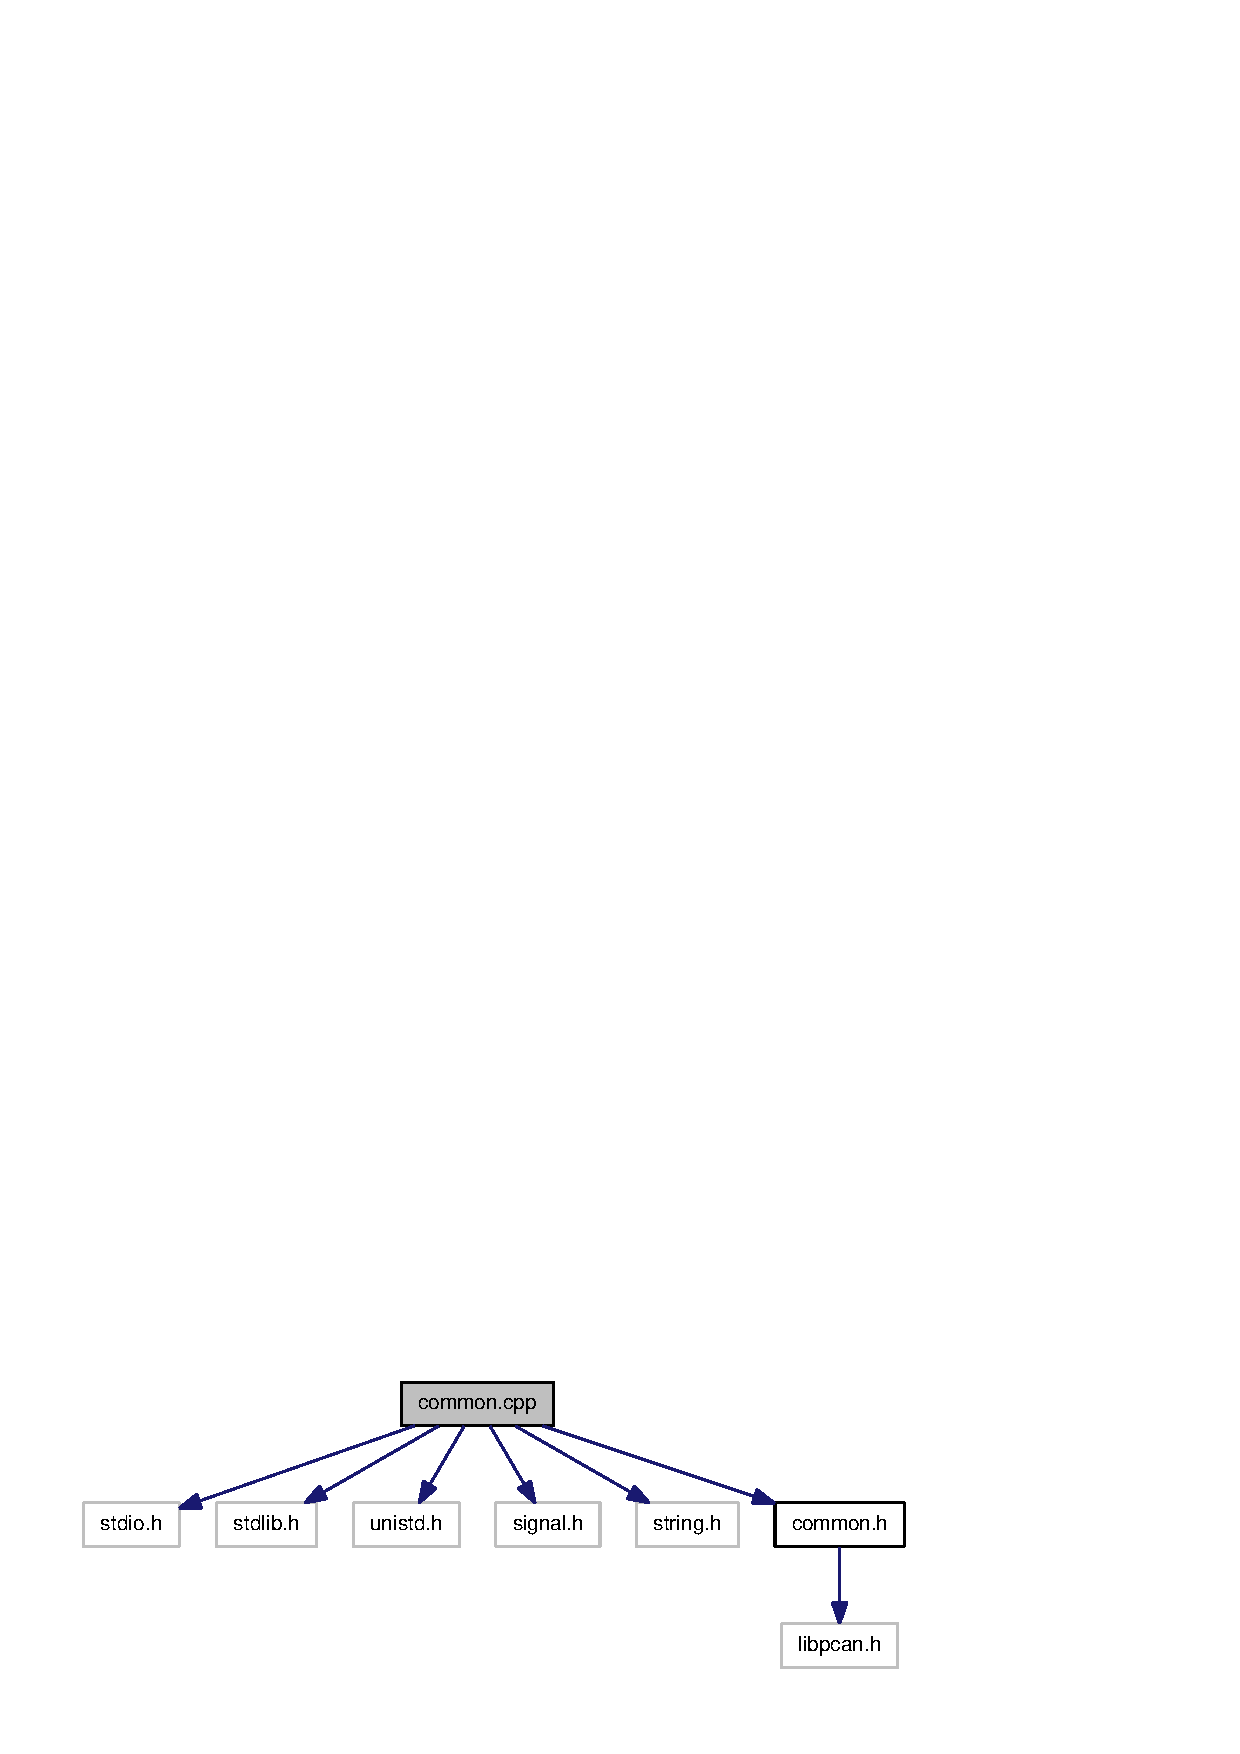
\includegraphics[width=350pt]{common_8cpp__incl}
\end{center}
\end{figure}
\subsection*{\-Functions}
\begin{DoxyCompactItemize}
\item 
void {\bf do\-\_\-exit} (int error)
\item 
char $\ast$ {\bf get\-Name\-Of\-Interface} (int n\-Type)
\item 
void {\bf print\-\_\-diag} (const char $\ast$prg\-Name)
\item 
void {\bf signal\-\_\-handler} (int signal)
\end{DoxyCompactItemize}


\subsection{\-Function \-Documentation}
\index{common.\-cpp@{common.\-cpp}!do\-\_\-exit@{do\-\_\-exit}}
\index{do\-\_\-exit@{do\-\_\-exit}!common.cpp@{common.\-cpp}}
\subsubsection[{do\-\_\-exit}]{\setlength{\rightskip}{0pt plus 5cm}void {\bf do\-\_\-exit} (
\begin{DoxyParamCaption}
\item[{int}]{error}
\end{DoxyParamCaption}
)}\label{common_8cpp_a6eae555086e24c8d918131cf9d18d205}
\-The function is based on the \doxyref{do\-\_\-exit()}{p.}{common_8cpp_a6eae555086e24c8d918131cf9d18d205} function from both the transmi-\/ and receivetest programs.

\-Definition at line 37 of file common.\-cpp.

\index{common.\-cpp@{common.\-cpp}!get\-Name\-Of\-Interface@{get\-Name\-Of\-Interface}}
\index{get\-Name\-Of\-Interface@{get\-Name\-Of\-Interface}!common.cpp@{common.\-cpp}}
\subsubsection[{get\-Name\-Of\-Interface}]{\setlength{\rightskip}{0pt plus 5cm}char$\ast$ {\bf get\-Name\-Of\-Interface} (
\begin{DoxyParamCaption}
\item[{int}]{n\-Type}
\end{DoxyParamCaption}
)}\label{common_8cpp_a84c56e815d950087c848a6044c3602b1}
\-The function is copied from the \doxyref{common.\-cpp}{p.}{common_8cpp} file used by both the transmi-\/ and receivetest

\-Definition at line 57 of file common.\-cpp.

\index{common.\-cpp@{common.\-cpp}!print\-\_\-diag@{print\-\_\-diag}}
\index{print\-\_\-diag@{print\-\_\-diag}!common.cpp@{common.\-cpp}}
\subsubsection[{print\-\_\-diag}]{\setlength{\rightskip}{0pt plus 5cm}void {\bf print\-\_\-diag} (
\begin{DoxyParamCaption}
\item[{const char $\ast$}]{prg\-Name}
\end{DoxyParamCaption}
)}\label{common_8cpp_ad9ddf38b3664f62c72f786d4af0ed067}
\-The function is copied from the \doxyref{common.\-cpp}{p.}{common_8cpp} file used by both the transmi-\/ and receivetest

\-Definition at line 80 of file common.\-cpp.

\index{common.\-cpp@{common.\-cpp}!signal\-\_\-handler@{signal\-\_\-handler}}
\index{signal\-\_\-handler@{signal\-\_\-handler}!common.cpp@{common.\-cpp}}
\subsubsection[{signal\-\_\-handler}]{\setlength{\rightskip}{0pt plus 5cm}void {\bf signal\-\_\-handler} (
\begin{DoxyParamCaption}
\item[{int}]{signal}
\end{DoxyParamCaption}
)}\label{common_8cpp_a3b527c56ed133ee6815bfbc625e757af}
\-The function is based on the \doxyref{signal\-\_\-handler()}{p.}{common_8cpp_a3b527c56ed133ee6815bfbc625e757af} function from the receivetest program.

\-Definition at line 26 of file common.\-cpp.


\section{common.\-h \-File \-Reference}
\label{common_8h}\index{common.\-h@{common.\-h}}
{\ttfamily \#include $<$libpcan.\-h$>$}\*
\-Include dependency graph for common.\-h\-:\nopagebreak
\begin{figure}[H]
\begin{center}
\leavevmode
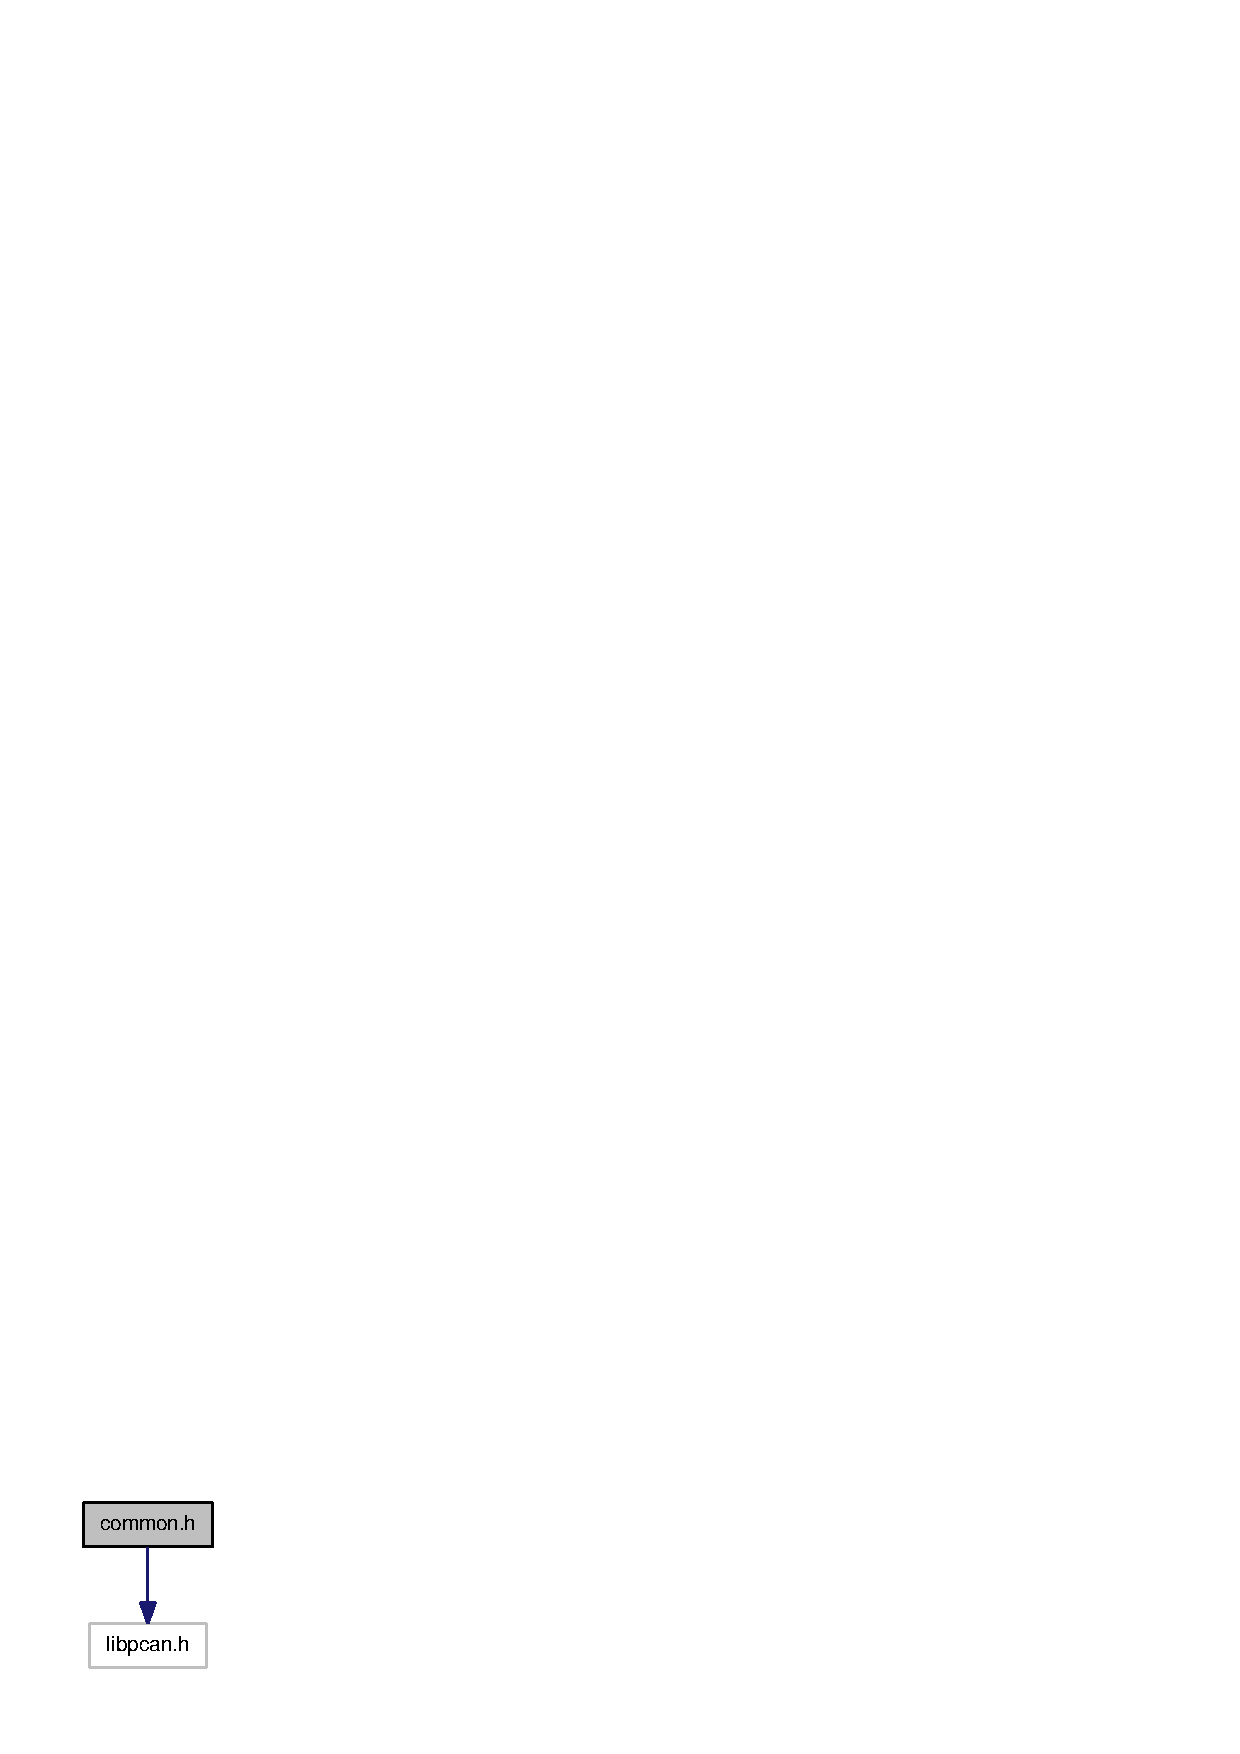
\includegraphics[width=106pt]{common_8h__incl}
\end{center}
\end{figure}
\-This graph shows which files directly or indirectly include this file\-:\nopagebreak
\begin{figure}[H]
\begin{center}
\leavevmode
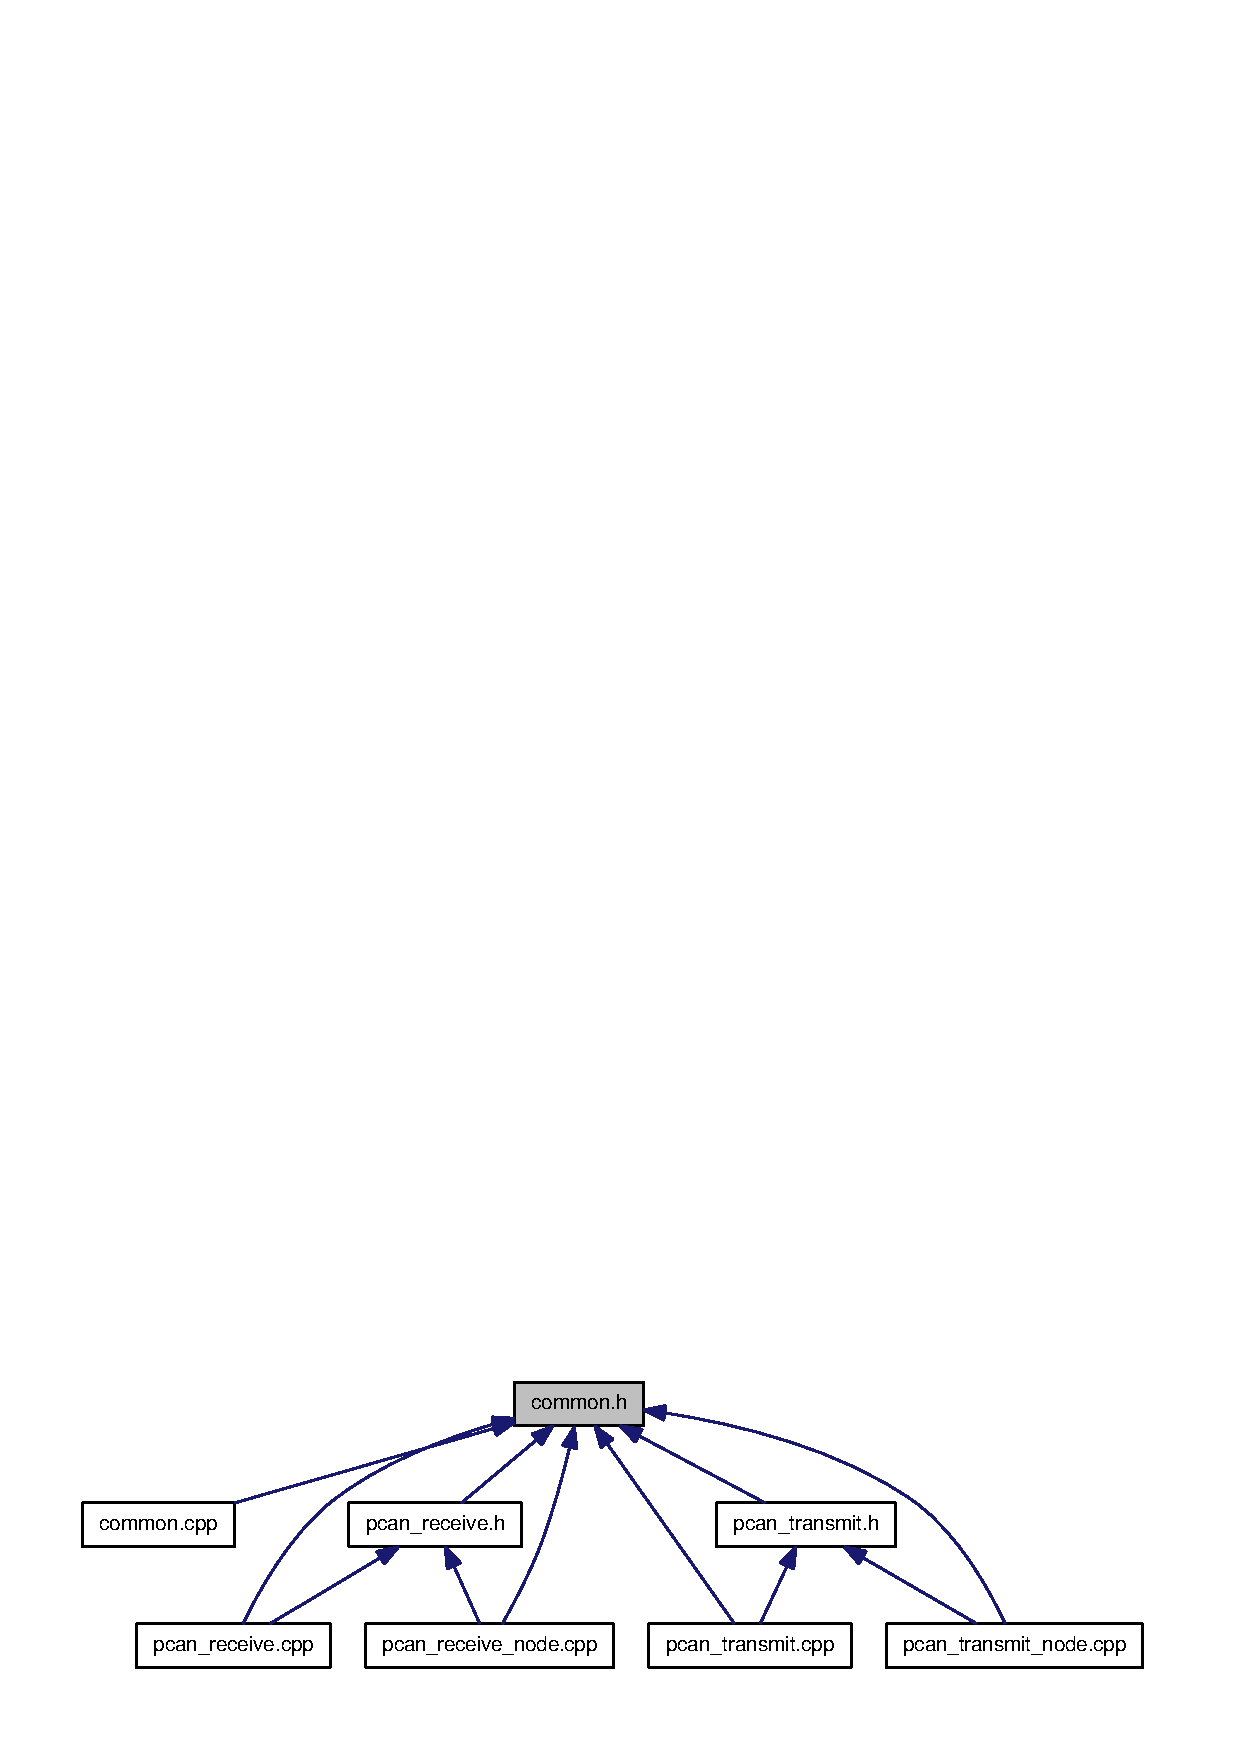
\includegraphics[width=350pt]{common_8h__dep__incl}
\end{center}
\end{figure}
\subsection*{\-Functions}
\begin{DoxyCompactItemize}
\item 
void {\bf do\-\_\-exit} (int error)
\item 
char $\ast$ {\bf get\-Name\-Of\-Interface} (int n\-Type)
\item 
void {\bf print\-\_\-diag} (const char $\ast$prg\-Name)
\item 
void {\bf signal\-\_\-handler} (int signal)
\end{DoxyCompactItemize}
\subsection*{\-Variables}
\begin{DoxyCompactItemize}
\item 
const char $\ast$ {\bf current\-\_\-release}
\item 
\-H\-A\-N\-D\-L\-E {\bf h}
\end{DoxyCompactItemize}


\subsection{\-Function \-Documentation}
\index{common.\-h@{common.\-h}!do\-\_\-exit@{do\-\_\-exit}}
\index{do\-\_\-exit@{do\-\_\-exit}!common.h@{common.\-h}}
\subsubsection[{do\-\_\-exit}]{\setlength{\rightskip}{0pt plus 5cm}void {\bf do\-\_\-exit} (
\begin{DoxyParamCaption}
\item[{int}]{error}
\end{DoxyParamCaption}
)}\label{common_8h_a6eae555086e24c8d918131cf9d18d205}
\-The function is based on the \doxyref{do\-\_\-exit()}{p.}{common_8cpp_a6eae555086e24c8d918131cf9d18d205} function from both the transmi-\/ and receivetest programs.

\-Definition at line 37 of file common.\-cpp.

\index{common.\-h@{common.\-h}!get\-Name\-Of\-Interface@{get\-Name\-Of\-Interface}}
\index{get\-Name\-Of\-Interface@{get\-Name\-Of\-Interface}!common.h@{common.\-h}}
\subsubsection[{get\-Name\-Of\-Interface}]{\setlength{\rightskip}{0pt plus 5cm}char$\ast$ {\bf get\-Name\-Of\-Interface} (
\begin{DoxyParamCaption}
\item[{int}]{n\-Type}
\end{DoxyParamCaption}
)}\label{common_8h_a84c56e815d950087c848a6044c3602b1}
\-The function is copied from the \doxyref{common.\-cpp}{p.}{common_8cpp} file used by both the transmi-\/ and receivetest

\-Definition at line 57 of file common.\-cpp.

\index{common.\-h@{common.\-h}!print\-\_\-diag@{print\-\_\-diag}}
\index{print\-\_\-diag@{print\-\_\-diag}!common.h@{common.\-h}}
\subsubsection[{print\-\_\-diag}]{\setlength{\rightskip}{0pt plus 5cm}void {\bf print\-\_\-diag} (
\begin{DoxyParamCaption}
\item[{const char $\ast$}]{prg\-Name}
\end{DoxyParamCaption}
)}\label{common_8h_ad9ddf38b3664f62c72f786d4af0ed067}
\-The function is copied from the \doxyref{common.\-cpp}{p.}{common_8cpp} file used by both the transmi-\/ and receivetest

\-Definition at line 80 of file common.\-cpp.

\index{common.\-h@{common.\-h}!signal\-\_\-handler@{signal\-\_\-handler}}
\index{signal\-\_\-handler@{signal\-\_\-handler}!common.h@{common.\-h}}
\subsubsection[{signal\-\_\-handler}]{\setlength{\rightskip}{0pt plus 5cm}void {\bf signal\-\_\-handler} (
\begin{DoxyParamCaption}
\item[{int}]{signal}
\end{DoxyParamCaption}
)}\label{common_8h_a3b527c56ed133ee6815bfbc625e757af}
\-The function is based on the \doxyref{signal\-\_\-handler()}{p.}{common_8cpp_a3b527c56ed133ee6815bfbc625e757af} function from the receivetest program.

\-Definition at line 26 of file common.\-cpp.



\subsection{\-Variable \-Documentation}
\index{common.\-h@{common.\-h}!current\-\_\-release@{current\-\_\-release}}
\index{current\-\_\-release@{current\-\_\-release}!common.h@{common.\-h}}
\subsubsection[{current\-\_\-release}]{\setlength{\rightskip}{0pt plus 5cm}const char$\ast$ {\bf current\-\_\-release}}\label{common_8h_ab70111b16fc3d1e36d0a598452c6f43c}


\-Definition at line 27 of file pcan\-\_\-receive\-\_\-node.\-cpp.

\index{common.\-h@{common.\-h}!h@{h}}
\index{h@{h}!common.h@{common.\-h}}
\subsubsection[{h}]{\setlength{\rightskip}{0pt plus 5cm}\-H\-A\-N\-D\-L\-E {\bf h}}\label{common_8h_a0182b2e472b8af2291079784ca8926c9}


\-Definition at line 26 of file pcan\-\_\-receive\-\_\-node.\-cpp.


\section{mainpage.\-dox \-File \-Reference}
\label{mainpage_8dox}\index{mainpage.\-dox@{mainpage.\-dox}}

\section{pcan\-\_\-receive.\-cpp \-File \-Reference}
\label{pcan__receive_8cpp}\index{pcan\-\_\-receive.\-cpp@{pcan\-\_\-receive.\-cpp}}
{\ttfamily \#include $<$stdio.\-h$>$}\*
{\ttfamily \#include $<$stdlib.\-h$>$}\*
{\ttfamily \#include $<$errno.\-h$>$}\*
{\ttfamily \#include $<$unistd.\-h$>$}\*
{\ttfamily \#include $<$signal.\-h$>$}\*
{\ttfamily \#include $<$string.\-h$>$}\*
{\ttfamily \#include $<$fcntl.\-h$>$}\*
{\ttfamily \#include $<$libpcan.\-h$>$}\*
{\ttfamily \#include \char`\"{}common.\-h\char`\"{}}\*
{\ttfamily \#include $<$ctype.\-h$>$}\*
{\ttfamily \#include \char`\"{}ros/ros.\-h\char`\"{}}\*
{\ttfamily \#include \char`\"{}std\-\_\-msgs/\-String.\-h\char`\"{}}\*
{\ttfamily \#include $<$sstream$>$}\*
{\ttfamily \#include \char`\"{}pcan\-\_\-receive.\-h\char`\"{}}\*
\-Include dependency graph for pcan\-\_\-receive.\-cpp\-:\nopagebreak
\begin{figure}[H]
\begin{center}
\leavevmode
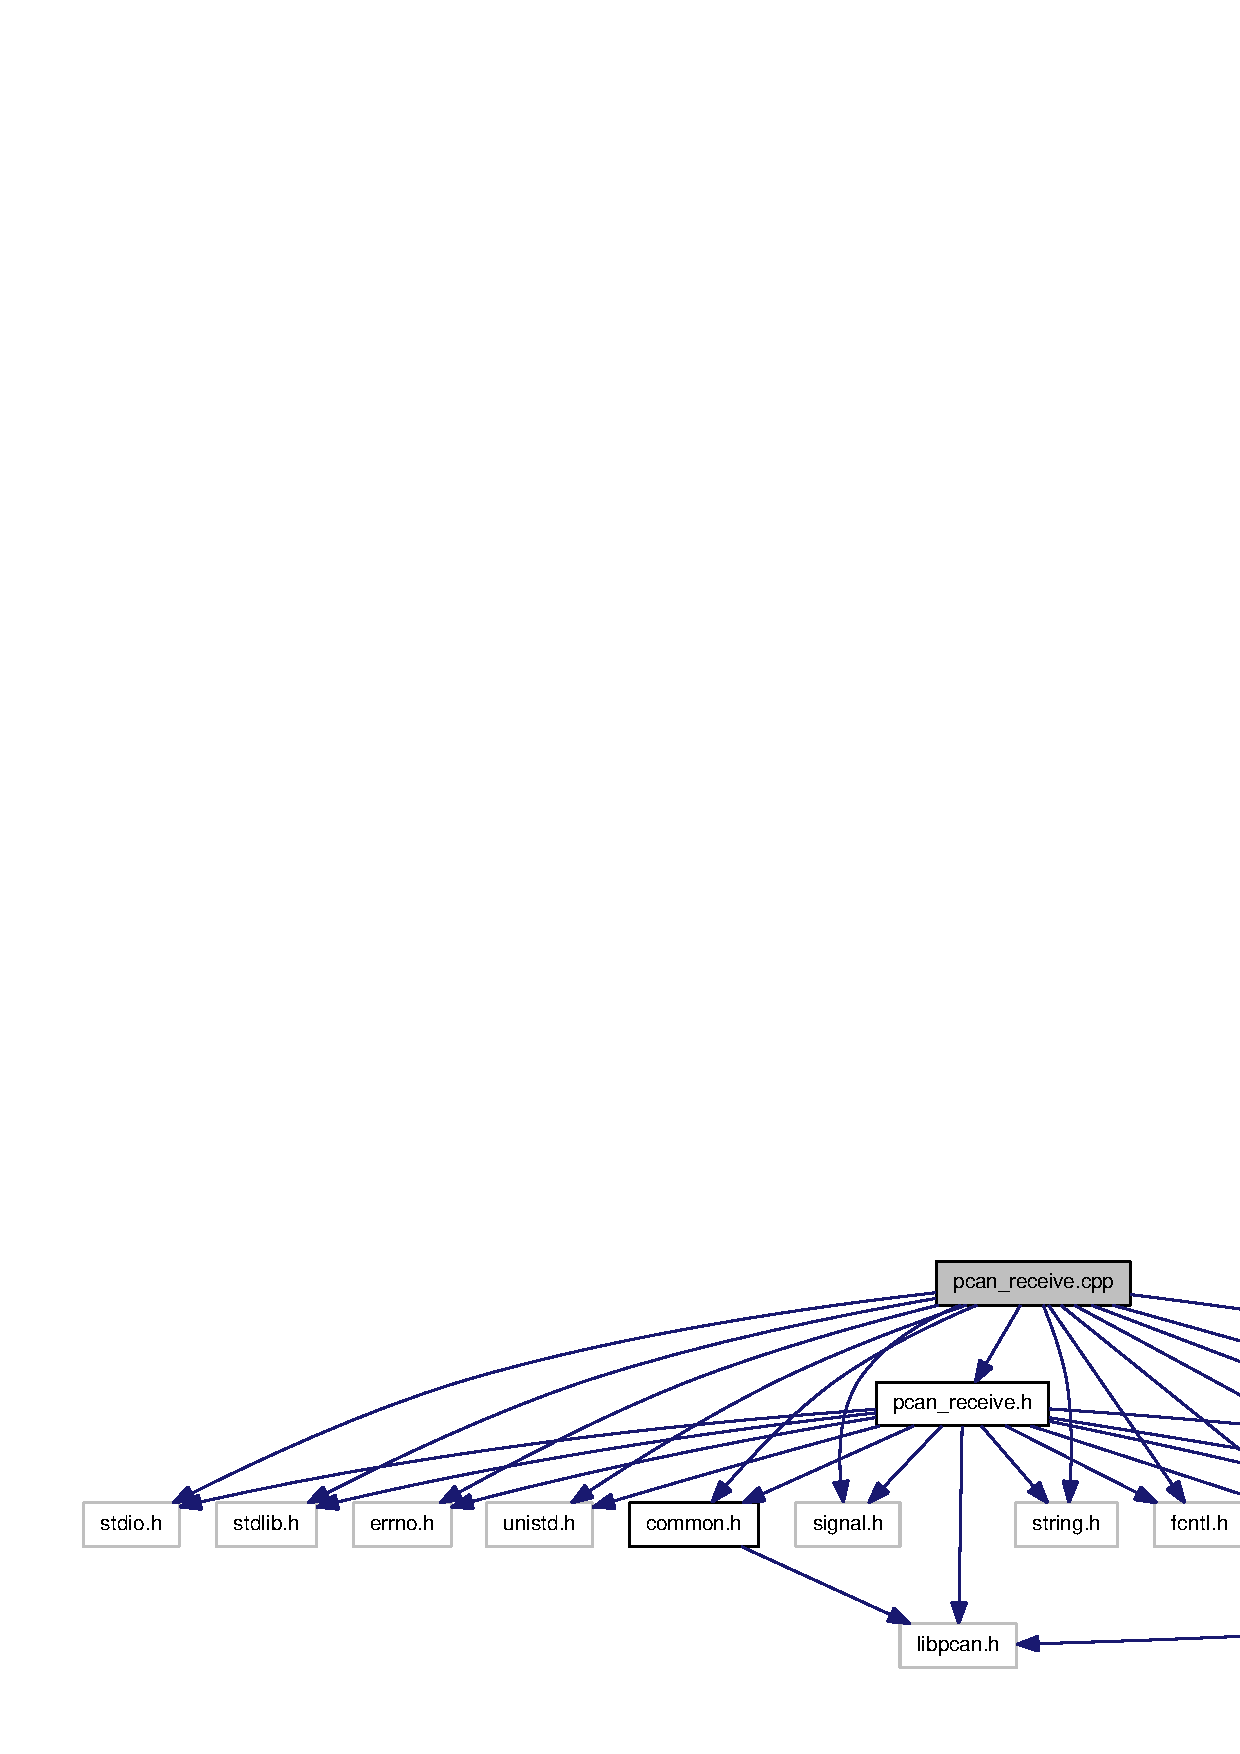
\includegraphics[width=350pt]{pcan__receive_8cpp__incl}
\end{center}
\end{figure}

\section{pcan\-\_\-receive.\-h \-File \-Reference}
\label{pcan__receive_8h}\index{pcan\-\_\-receive.\-h@{pcan\-\_\-receive.\-h}}
{\ttfamily \#include $<$stdio.\-h$>$}\*
{\ttfamily \#include $<$stdlib.\-h$>$}\*
{\ttfamily \#include $<$errno.\-h$>$}\*
{\ttfamily \#include $<$unistd.\-h$>$}\*
{\ttfamily \#include $<$signal.\-h$>$}\*
{\ttfamily \#include $<$string.\-h$>$}\*
{\ttfamily \#include $<$fcntl.\-h$>$}\*
{\ttfamily \#include $<$libpcan.\-h$>$}\*
{\ttfamily \#include \char`\"{}common.\-h\char`\"{}}\*
{\ttfamily \#include $<$ctype.\-h$>$}\*
{\ttfamily \#include \char`\"{}ros/ros.\-h\char`\"{}}\*
{\ttfamily \#include \char`\"{}std\-\_\-msgs/\-String.\-h\char`\"{}}\*
{\ttfamily \#include $<$sstream$>$}\*
\-Include dependency graph for pcan\-\_\-receive.\-h\-:\nopagebreak
\begin{figure}[H]
\begin{center}
\leavevmode
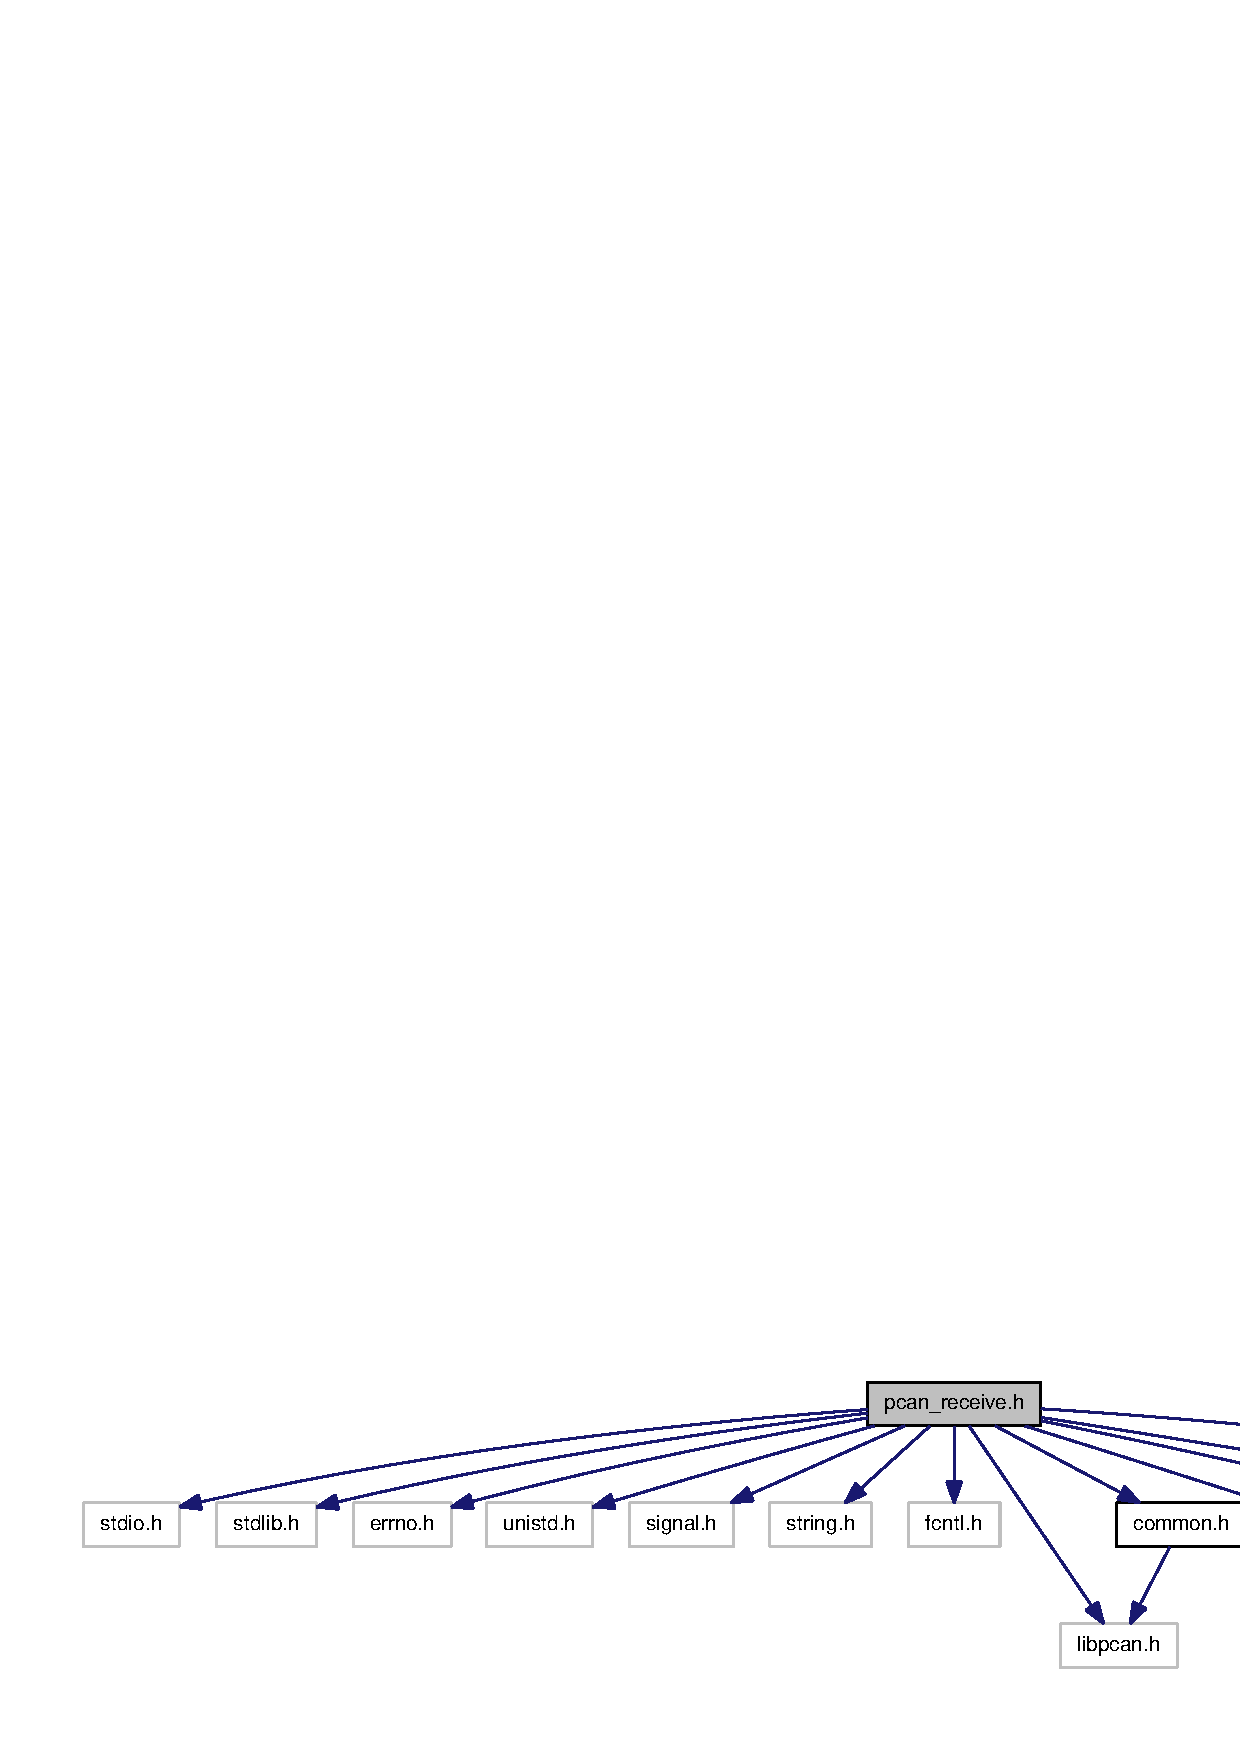
\includegraphics[width=350pt]{pcan__receive_8h__incl}
\end{center}
\end{figure}
\-This graph shows which files directly or indirectly include this file\-:\nopagebreak
\begin{figure}[H]
\begin{center}
\leavevmode
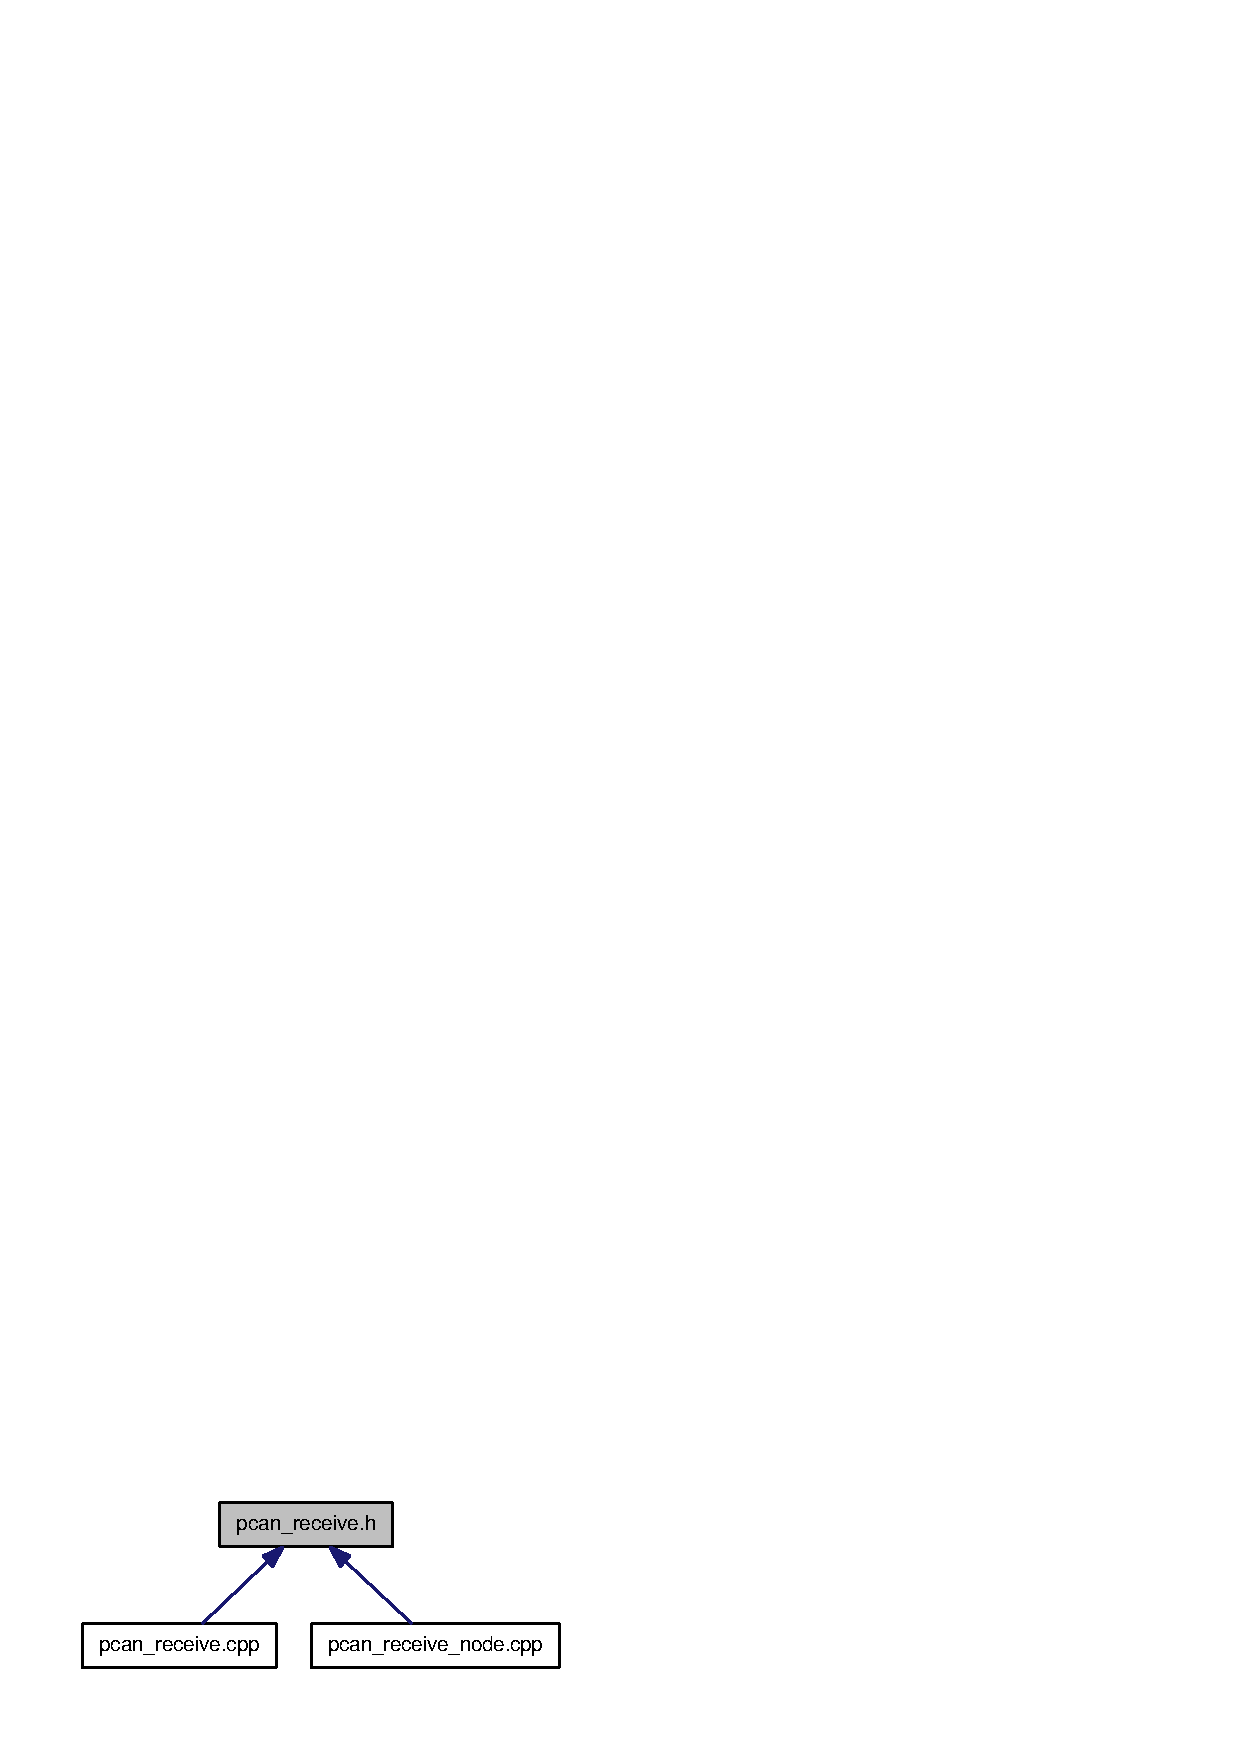
\includegraphics[width=272pt]{pcan__receive_8h__dep__incl}
\end{center}
\end{figure}
\subsection*{\-Classes}
\begin{DoxyCompactItemize}
\item 
class {\bf pcan\-\_\-receive}
\end{DoxyCompactItemize}
\subsection*{\-Defines}
\begin{DoxyCompactItemize}
\item 
\#define {\bf \-C\-U\-R\-R\-E\-N\-T\-\_\-\-R\-E\-L\-E\-A\-S\-E}~\char`\"{}\-Release\-\_\-20090203\-\_\-n\char`\"{}
\item 
\#define {\bf \-D\-E\-F\-A\-U\-L\-T\-\_\-\-N\-O\-D\-E}~\char`\"{}/dev/pcan32\char`\"{}
\end{DoxyCompactItemize}


\subsection{\-Define \-Documentation}
\index{pcan\-\_\-receive.\-h@{pcan\-\_\-receive.\-h}!\-C\-U\-R\-R\-E\-N\-T\-\_\-\-R\-E\-L\-E\-A\-S\-E@{\-C\-U\-R\-R\-E\-N\-T\-\_\-\-R\-E\-L\-E\-A\-S\-E}}
\index{\-C\-U\-R\-R\-E\-N\-T\-\_\-\-R\-E\-L\-E\-A\-S\-E@{\-C\-U\-R\-R\-E\-N\-T\-\_\-\-R\-E\-L\-E\-A\-S\-E}!pcan_receive.h@{pcan\-\_\-receive.\-h}}
\subsubsection[{\-C\-U\-R\-R\-E\-N\-T\-\_\-\-R\-E\-L\-E\-A\-S\-E}]{\setlength{\rightskip}{0pt plus 5cm}\#define {\bf \-C\-U\-R\-R\-E\-N\-T\-\_\-\-R\-E\-L\-E\-A\-S\-E}~\char`\"{}\-Release\-\_\-20090203\-\_\-n\char`\"{}}\label{pcan__receive_8h_a83a4c9c8303948a33b0bc5050142643a}


\-Definition at line 22 of file pcan\-\_\-receive.\-h.

\index{pcan\-\_\-receive.\-h@{pcan\-\_\-receive.\-h}!\-D\-E\-F\-A\-U\-L\-T\-\_\-\-N\-O\-D\-E@{\-D\-E\-F\-A\-U\-L\-T\-\_\-\-N\-O\-D\-E}}
\index{\-D\-E\-F\-A\-U\-L\-T\-\_\-\-N\-O\-D\-E@{\-D\-E\-F\-A\-U\-L\-T\-\_\-\-N\-O\-D\-E}!pcan_receive.h@{pcan\-\_\-receive.\-h}}
\subsubsection[{\-D\-E\-F\-A\-U\-L\-T\-\_\-\-N\-O\-D\-E}]{\setlength{\rightskip}{0pt plus 5cm}\#define {\bf \-D\-E\-F\-A\-U\-L\-T\-\_\-\-N\-O\-D\-E}~\char`\"{}/dev/pcan32\char`\"{}}\label{pcan__receive_8h_a7ce36d8e87af0db87c0d228a64201e35}


\-Definition at line 21 of file pcan\-\_\-receive.\-h.


\section{pcan\-\_\-receive\-\_\-node.\-cpp \-File \-Reference}
\label{pcan__receive__node_8cpp}\index{pcan\-\_\-receive\-\_\-node.\-cpp@{pcan\-\_\-receive\-\_\-node.\-cpp}}
{\ttfamily \#include $<$stdio.\-h$>$}\*
{\ttfamily \#include $<$stdlib.\-h$>$}\*
{\ttfamily \#include $<$errno.\-h$>$}\*
{\ttfamily \#include $<$unistd.\-h$>$}\*
{\ttfamily \#include $<$signal.\-h$>$}\*
{\ttfamily \#include $<$string.\-h$>$}\*
{\ttfamily \#include $<$fcntl.\-h$>$}\*
{\ttfamily \#include $<$libpcan.\-h$>$}\*
{\ttfamily \#include $<$ctype.\-h$>$}\*
{\ttfamily \#include \char`\"{}common.\-h\char`\"{}}\*
{\ttfamily \#include \char`\"{}pcan\-\_\-receive.\-h\char`\"{}}\*
{\ttfamily \#include \char`\"{}ros/ros.\-h\char`\"{}}\*
{\ttfamily \#include \char`\"{}std\-\_\-msgs/\-String.\-h\char`\"{}}\*
{\ttfamily \#include $<$sstream$>$}\*
\-Include dependency graph for pcan\-\_\-receive\-\_\-node.\-cpp\-:\nopagebreak
\begin{figure}[H]
\begin{center}
\leavevmode
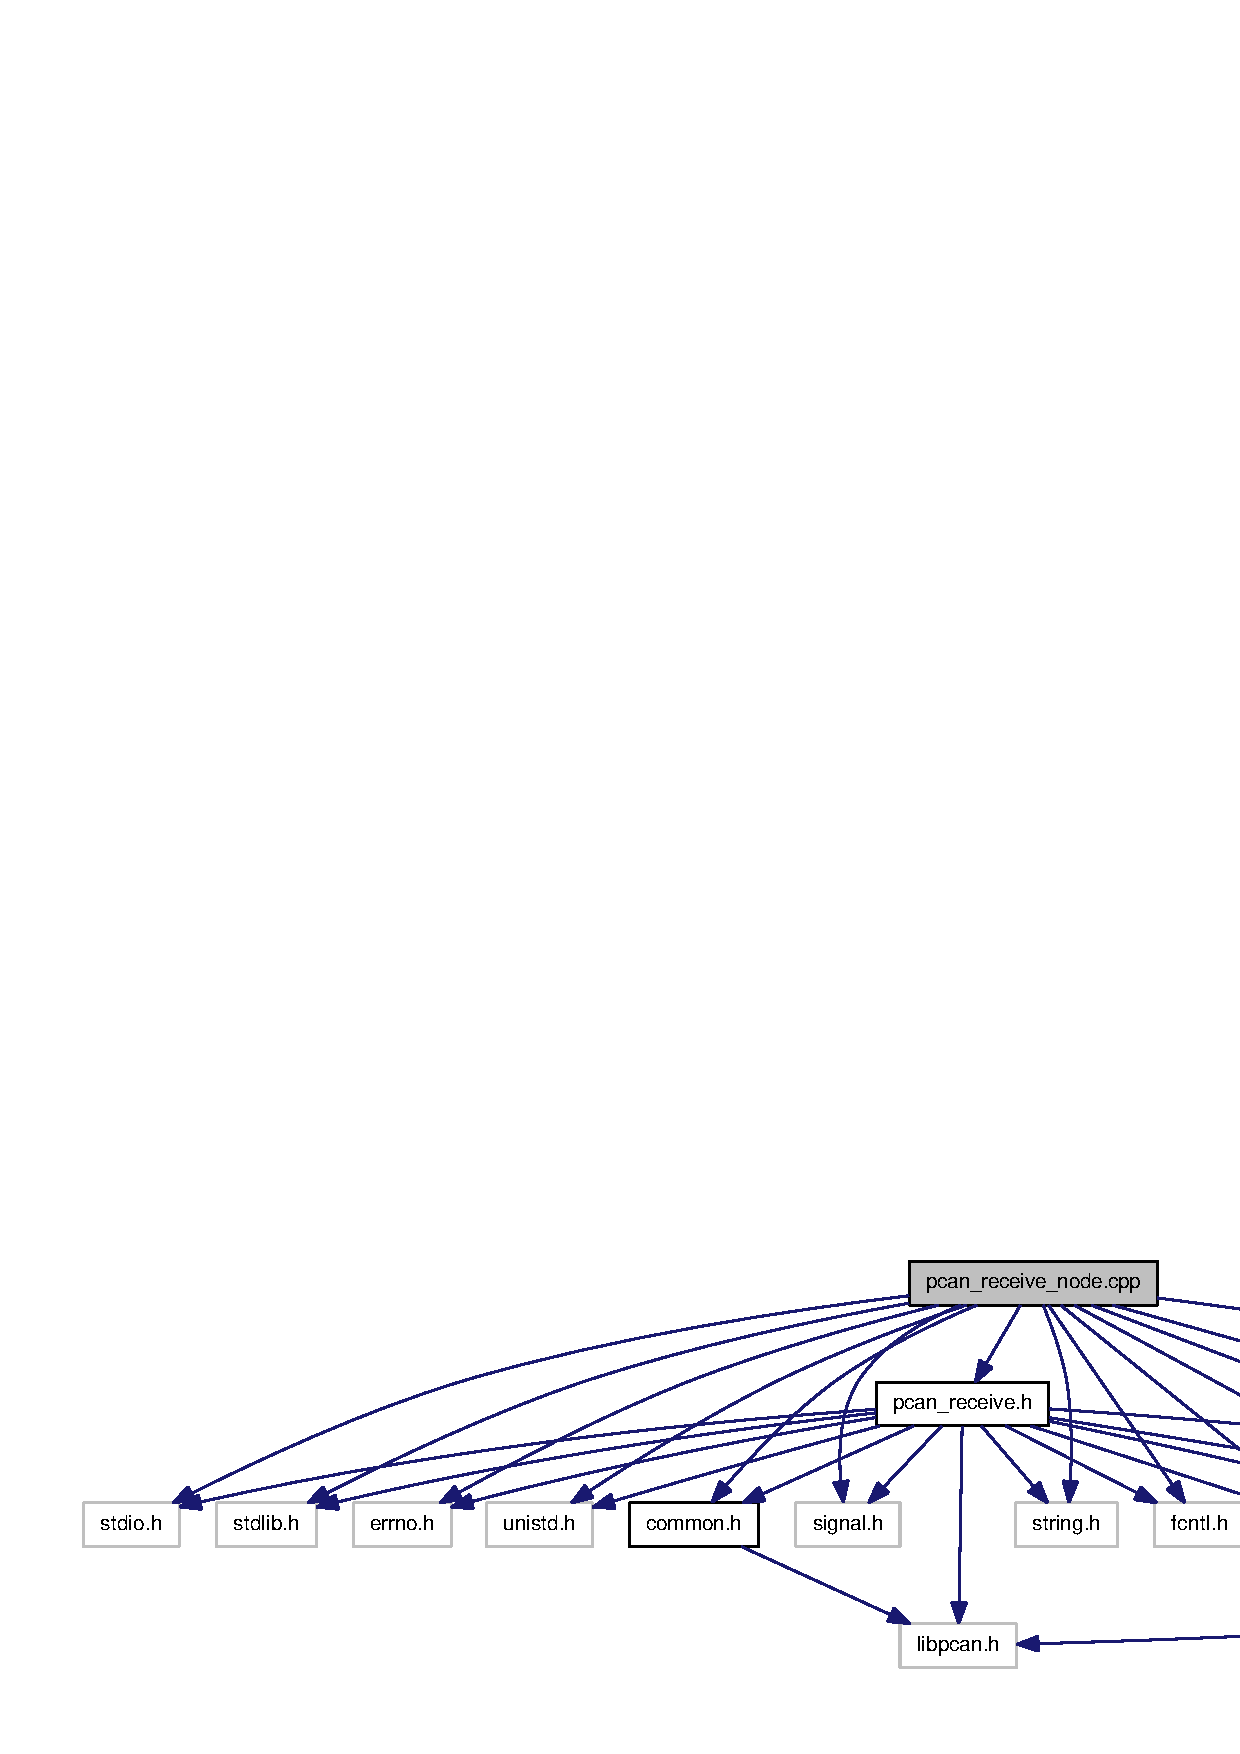
\includegraphics[width=350pt]{pcan__receive__node_8cpp__incl}
\end{center}
\end{figure}
\subsection*{\-Defines}
\begin{DoxyCompactItemize}
\item 
\#define {\bf \-C\-U\-R\-R\-E\-N\-T\-\_\-\-R\-E\-L\-E\-A\-S\-E}~\char`\"{}\-Release\-\_\-20090203\-\_\-n\char`\"{}
\item 
\#define {\bf \-D\-E\-F\-A\-U\-L\-T\-\_\-\-N\-O\-D\-E}~\char`\"{}/dev/pcan32\char`\"{}
\end{DoxyCompactItemize}
\subsection*{\-Functions}
\begin{DoxyCompactItemize}
\item 
int {\bf main} (int argc, char $\ast$$\ast$argv)
\end{DoxyCompactItemize}
\subsection*{\-Variables}
\begin{DoxyCompactItemize}
\item 
const char $\ast$ {\bf current\-\_\-release}
\item 
\-H\-A\-N\-D\-L\-E {\bf h}
\end{DoxyCompactItemize}


\subsection{\-Define \-Documentation}
\index{pcan\-\_\-receive\-\_\-node.\-cpp@{pcan\-\_\-receive\-\_\-node.\-cpp}!\-C\-U\-R\-R\-E\-N\-T\-\_\-\-R\-E\-L\-E\-A\-S\-E@{\-C\-U\-R\-R\-E\-N\-T\-\_\-\-R\-E\-L\-E\-A\-S\-E}}
\index{\-C\-U\-R\-R\-E\-N\-T\-\_\-\-R\-E\-L\-E\-A\-S\-E@{\-C\-U\-R\-R\-E\-N\-T\-\_\-\-R\-E\-L\-E\-A\-S\-E}!pcan_receive_node.cpp@{pcan\-\_\-receive\-\_\-node.\-cpp}}
\subsubsection[{\-C\-U\-R\-R\-E\-N\-T\-\_\-\-R\-E\-L\-E\-A\-S\-E}]{\setlength{\rightskip}{0pt plus 5cm}\#define {\bf \-C\-U\-R\-R\-E\-N\-T\-\_\-\-R\-E\-L\-E\-A\-S\-E}~\char`\"{}\-Release\-\_\-20090203\-\_\-n\char`\"{}}\label{pcan__receive__node_8cpp_a83a4c9c8303948a33b0bc5050142643a}


\-Definition at line 22 of file pcan\-\_\-receive\-\_\-node.\-cpp.

\index{pcan\-\_\-receive\-\_\-node.\-cpp@{pcan\-\_\-receive\-\_\-node.\-cpp}!\-D\-E\-F\-A\-U\-L\-T\-\_\-\-N\-O\-D\-E@{\-D\-E\-F\-A\-U\-L\-T\-\_\-\-N\-O\-D\-E}}
\index{\-D\-E\-F\-A\-U\-L\-T\-\_\-\-N\-O\-D\-E@{\-D\-E\-F\-A\-U\-L\-T\-\_\-\-N\-O\-D\-E}!pcan_receive_node.cpp@{pcan\-\_\-receive\-\_\-node.\-cpp}}
\subsubsection[{\-D\-E\-F\-A\-U\-L\-T\-\_\-\-N\-O\-D\-E}]{\setlength{\rightskip}{0pt plus 5cm}\#define {\bf \-D\-E\-F\-A\-U\-L\-T\-\_\-\-N\-O\-D\-E}~\char`\"{}/dev/pcan32\char`\"{}}\label{pcan__receive__node_8cpp_a7ce36d8e87af0db87c0d228a64201e35}


\-Definition at line 21 of file pcan\-\_\-receive\-\_\-node.\-cpp.



\subsection{\-Function \-Documentation}
\index{pcan\-\_\-receive\-\_\-node.\-cpp@{pcan\-\_\-receive\-\_\-node.\-cpp}!main@{main}}
\index{main@{main}!pcan_receive_node.cpp@{pcan\-\_\-receive\-\_\-node.\-cpp}}
\subsubsection[{main}]{\setlength{\rightskip}{0pt plus 5cm}int {\bf main} (
\begin{DoxyParamCaption}
\item[{int}]{argc, }
\item[{char $\ast$$\ast$}]{argv}
\end{DoxyParamCaption}
)}\label{pcan__receive__node_8cpp_a3c04138a5bfe5d72780bb7e82a18e627}
\-The \doxyref{main()}{p.}{pcan__receive__node_8cpp_a3c04138a5bfe5d72780bb7e82a18e627} function only initiates a \-R\-O\-S node, creates and initializes a \doxyref{pcan\-\_\-receive}{p.}{classpcan__receive} object instance, sets two signal handlers and starts to loop.

\-Definition at line 30 of file pcan\-\_\-receive\-\_\-node.\-cpp.



\subsection{\-Variable \-Documentation}
\index{pcan\-\_\-receive\-\_\-node.\-cpp@{pcan\-\_\-receive\-\_\-node.\-cpp}!current\-\_\-release@{current\-\_\-release}}
\index{current\-\_\-release@{current\-\_\-release}!pcan_receive_node.cpp@{pcan\-\_\-receive\-\_\-node.\-cpp}}
\subsubsection[{current\-\_\-release}]{\setlength{\rightskip}{0pt plus 5cm}const char$\ast$ {\bf current\-\_\-release}}\label{pcan__receive__node_8cpp_ab70111b16fc3d1e36d0a598452c6f43c}


\-Definition at line 27 of file pcan\-\_\-receive\-\_\-node.\-cpp.

\index{pcan\-\_\-receive\-\_\-node.\-cpp@{pcan\-\_\-receive\-\_\-node.\-cpp}!h@{h}}
\index{h@{h}!pcan_receive_node.cpp@{pcan\-\_\-receive\-\_\-node.\-cpp}}
\subsubsection[{h}]{\setlength{\rightskip}{0pt plus 5cm}\-H\-A\-N\-D\-L\-E {\bf h}}\label{pcan__receive__node_8cpp_a0182b2e472b8af2291079784ca8926c9}


\-Definition at line 26 of file pcan\-\_\-receive\-\_\-node.\-cpp.


\section{pcan\-\_\-transmit.\-cpp \-File \-Reference}
\label{pcan__transmit_8cpp}\index{pcan\-\_\-transmit.\-cpp@{pcan\-\_\-transmit.\-cpp}}
{\ttfamily \#include $<$stdio.\-h$>$}\*
{\ttfamily \#include $<$stdlib.\-h$>$}\*
{\ttfamily \#include $<$errno.\-h$>$}\*
{\ttfamily \#include $<$unistd.\-h$>$}\*
{\ttfamily \#include $<$signal.\-h$>$}\*
{\ttfamily \#include $<$string.\-h$>$}\*
{\ttfamily \#include $<$fcntl.\-h$>$}\*
{\ttfamily \#include $<$libpcan.\-h$>$}\*
{\ttfamily \#include \char`\"{}common.\-h\char`\"{}}\*
{\ttfamily \#include $<$ctype.\-h$>$}\*
{\ttfamily \#include \char`\"{}ros/ros.\-h\char`\"{}}\*
{\ttfamily \#include \char`\"{}std\-\_\-msgs/\-String.\-h\char`\"{}}\*
{\ttfamily \#include $<$sstream$>$}\*
{\ttfamily \#include \char`\"{}pcan\-\_\-transmit.\-h\char`\"{}}\*
\-Include dependency graph for pcan\-\_\-transmit.\-cpp\-:\nopagebreak
\begin{figure}[H]
\begin{center}
\leavevmode
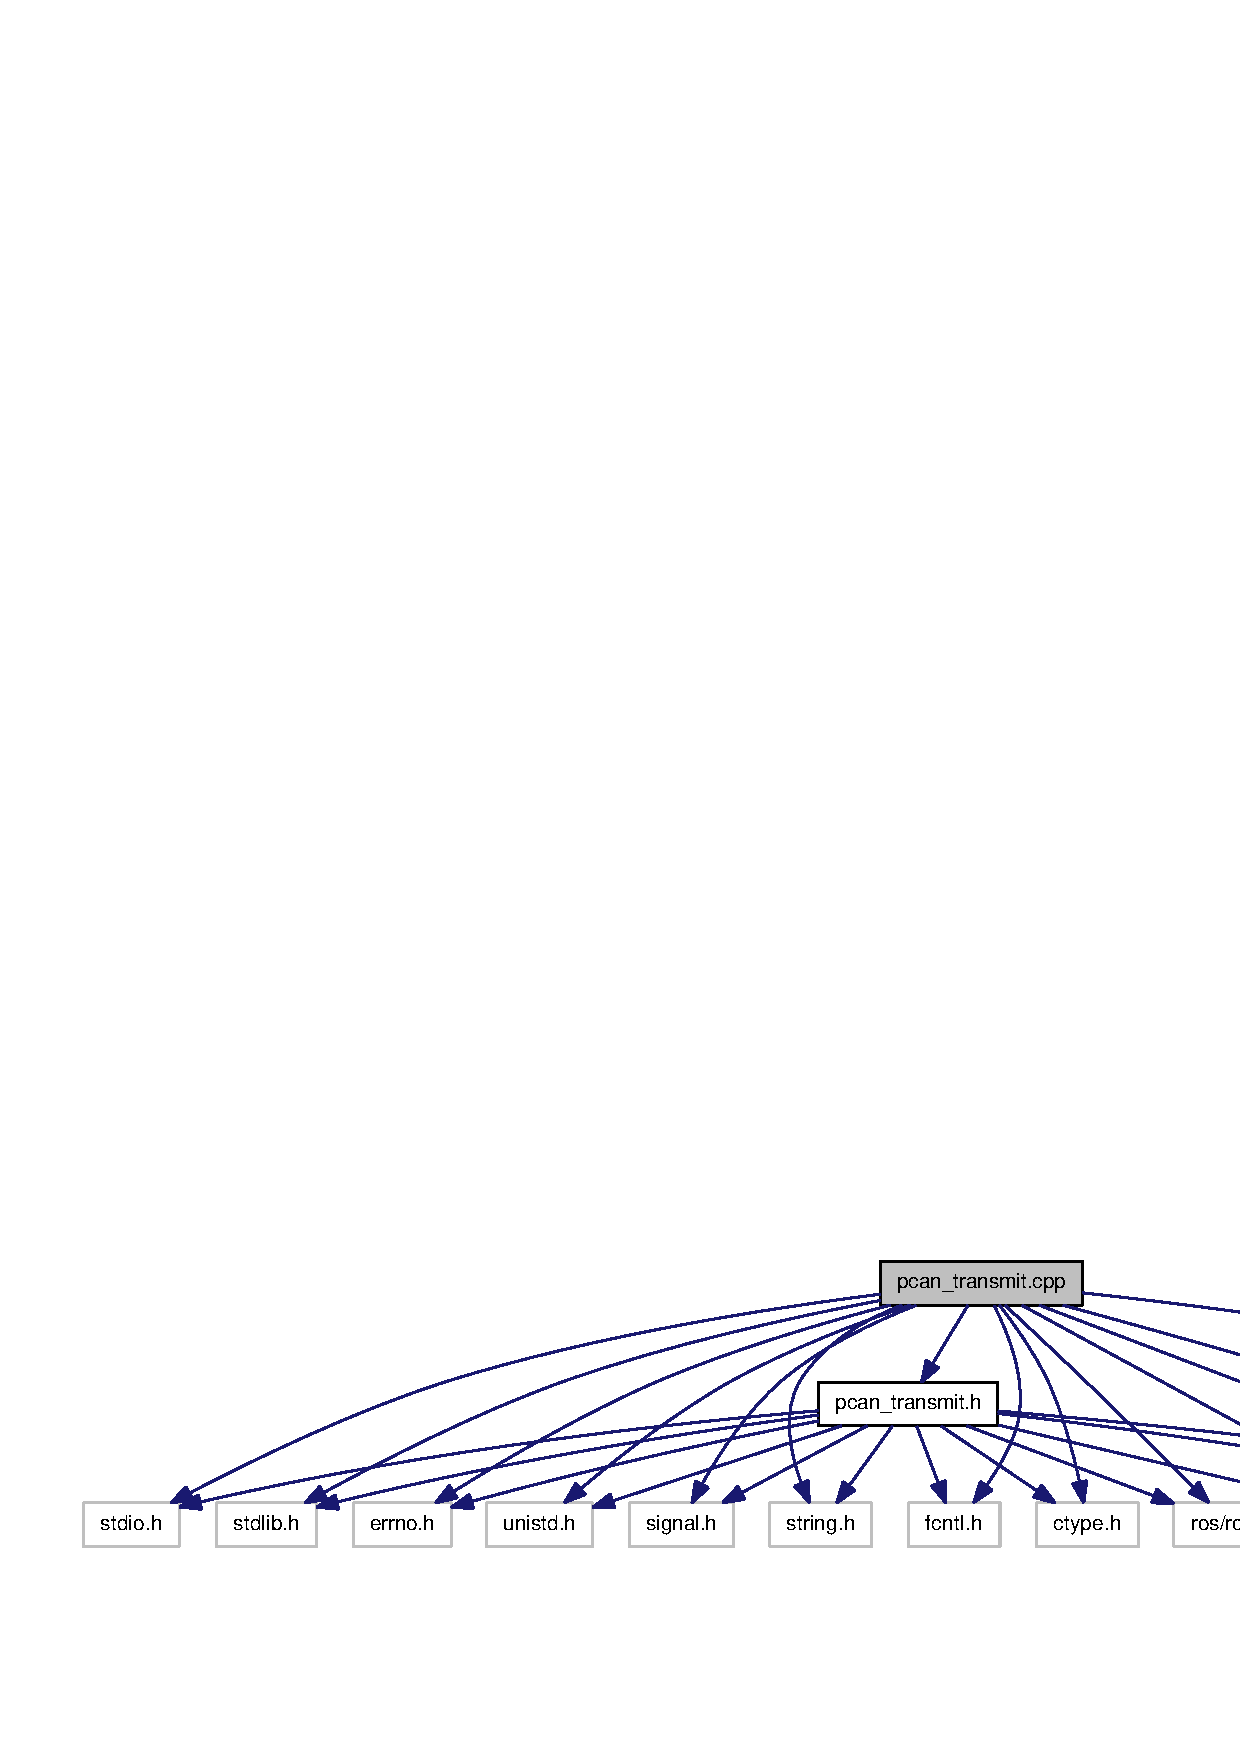
\includegraphics[width=350pt]{pcan__transmit_8cpp__incl}
\end{center}
\end{figure}

\section{pcan\-\_\-transmit.\-h \-File \-Reference}
\label{pcan__transmit_8h}\index{pcan\-\_\-transmit.\-h@{pcan\-\_\-transmit.\-h}}
{\ttfamily \#include $<$stdio.\-h$>$}\*
{\ttfamily \#include $<$stdlib.\-h$>$}\*
{\ttfamily \#include $<$errno.\-h$>$}\*
{\ttfamily \#include $<$unistd.\-h$>$}\*
{\ttfamily \#include $<$signal.\-h$>$}\*
{\ttfamily \#include $<$string.\-h$>$}\*
{\ttfamily \#include $<$fcntl.\-h$>$}\*
{\ttfamily \#include \char`\"{}common.\-h\char`\"{}}\*
{\ttfamily \#include $<$ctype.\-h$>$}\*
{\ttfamily \#include \char`\"{}ros/ros.\-h\char`\"{}}\*
{\ttfamily \#include \char`\"{}std\-\_\-msgs/\-String.\-h\char`\"{}}\*
{\ttfamily \#include $<$sstream$>$}\*
\-Include dependency graph for pcan\-\_\-transmit.\-h\-:\nopagebreak
\begin{figure}[H]
\begin{center}
\leavevmode
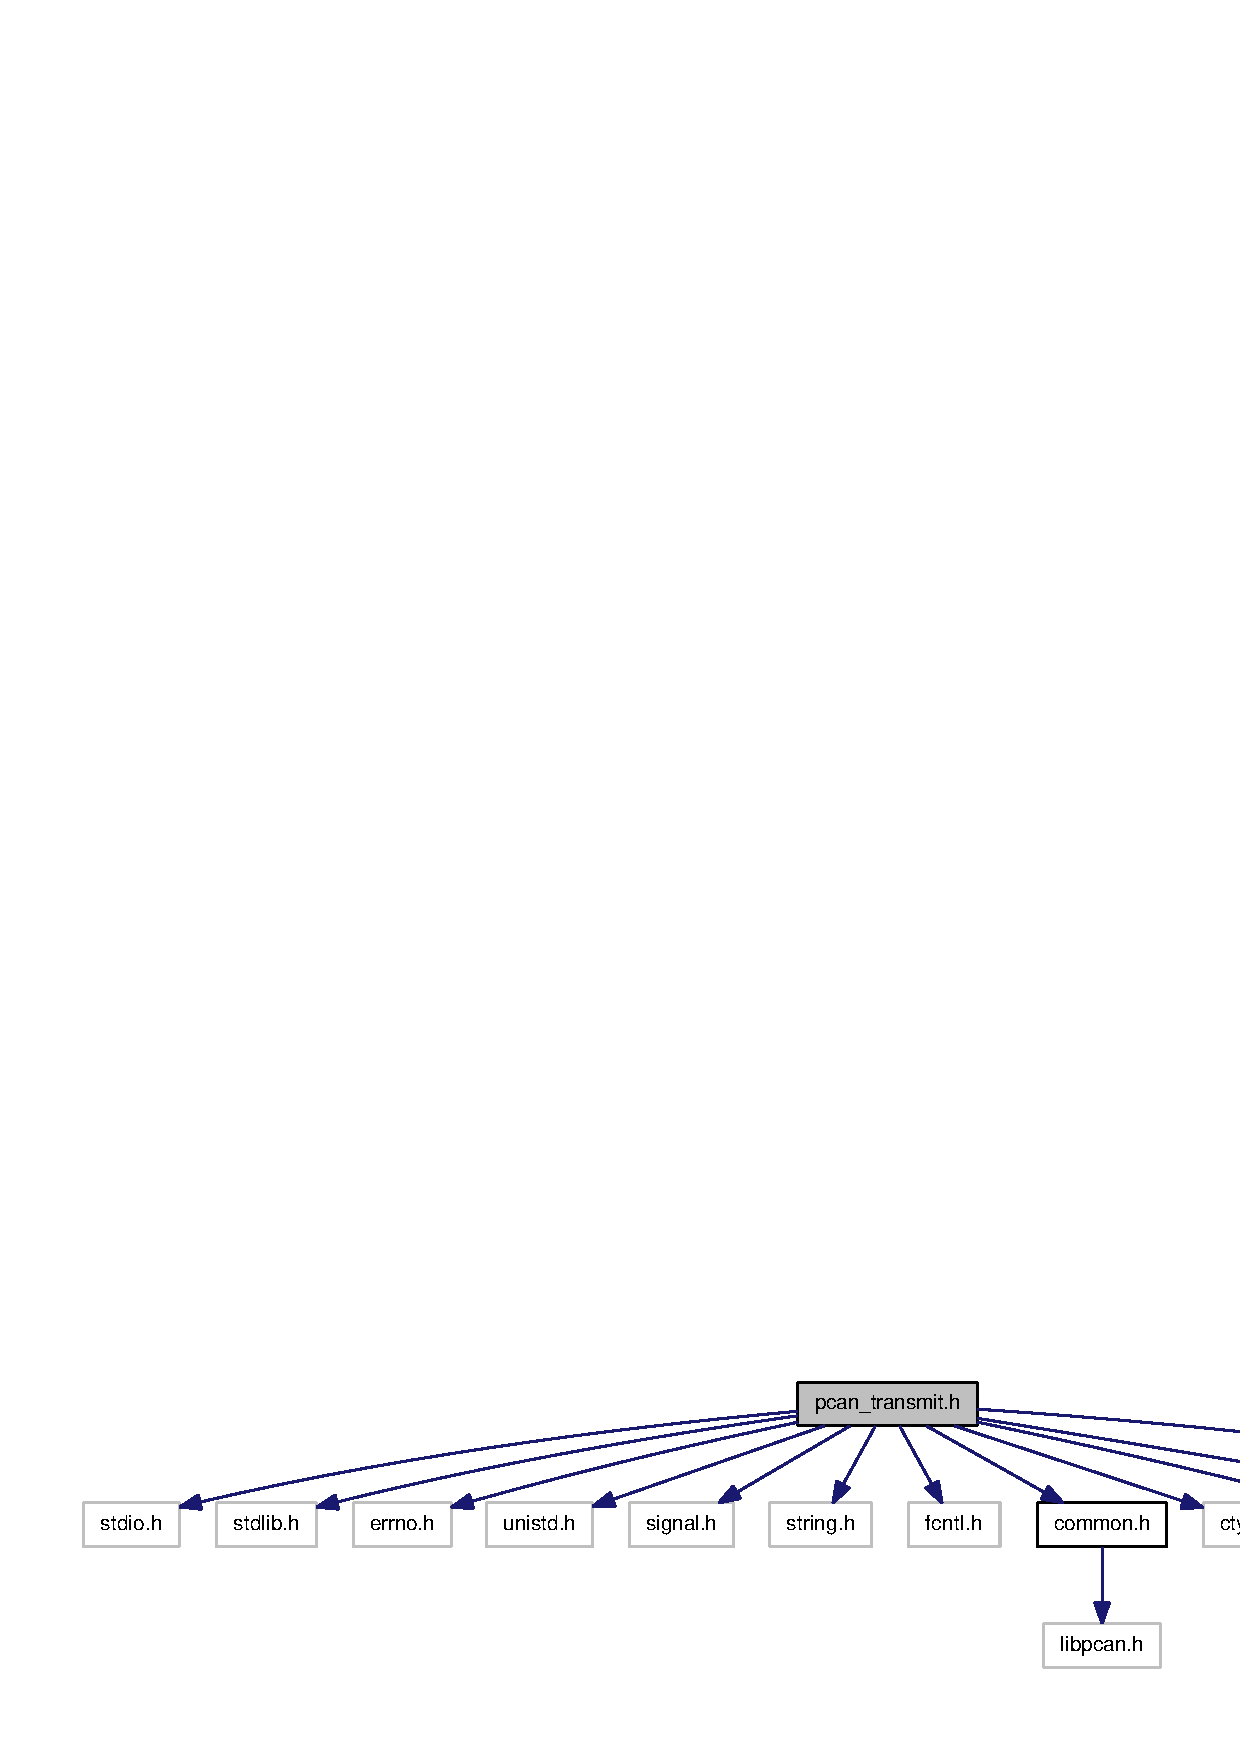
\includegraphics[width=350pt]{pcan__transmit_8h__incl}
\end{center}
\end{figure}
\-This graph shows which files directly or indirectly include this file\-:\nopagebreak
\begin{figure}[H]
\begin{center}
\leavevmode
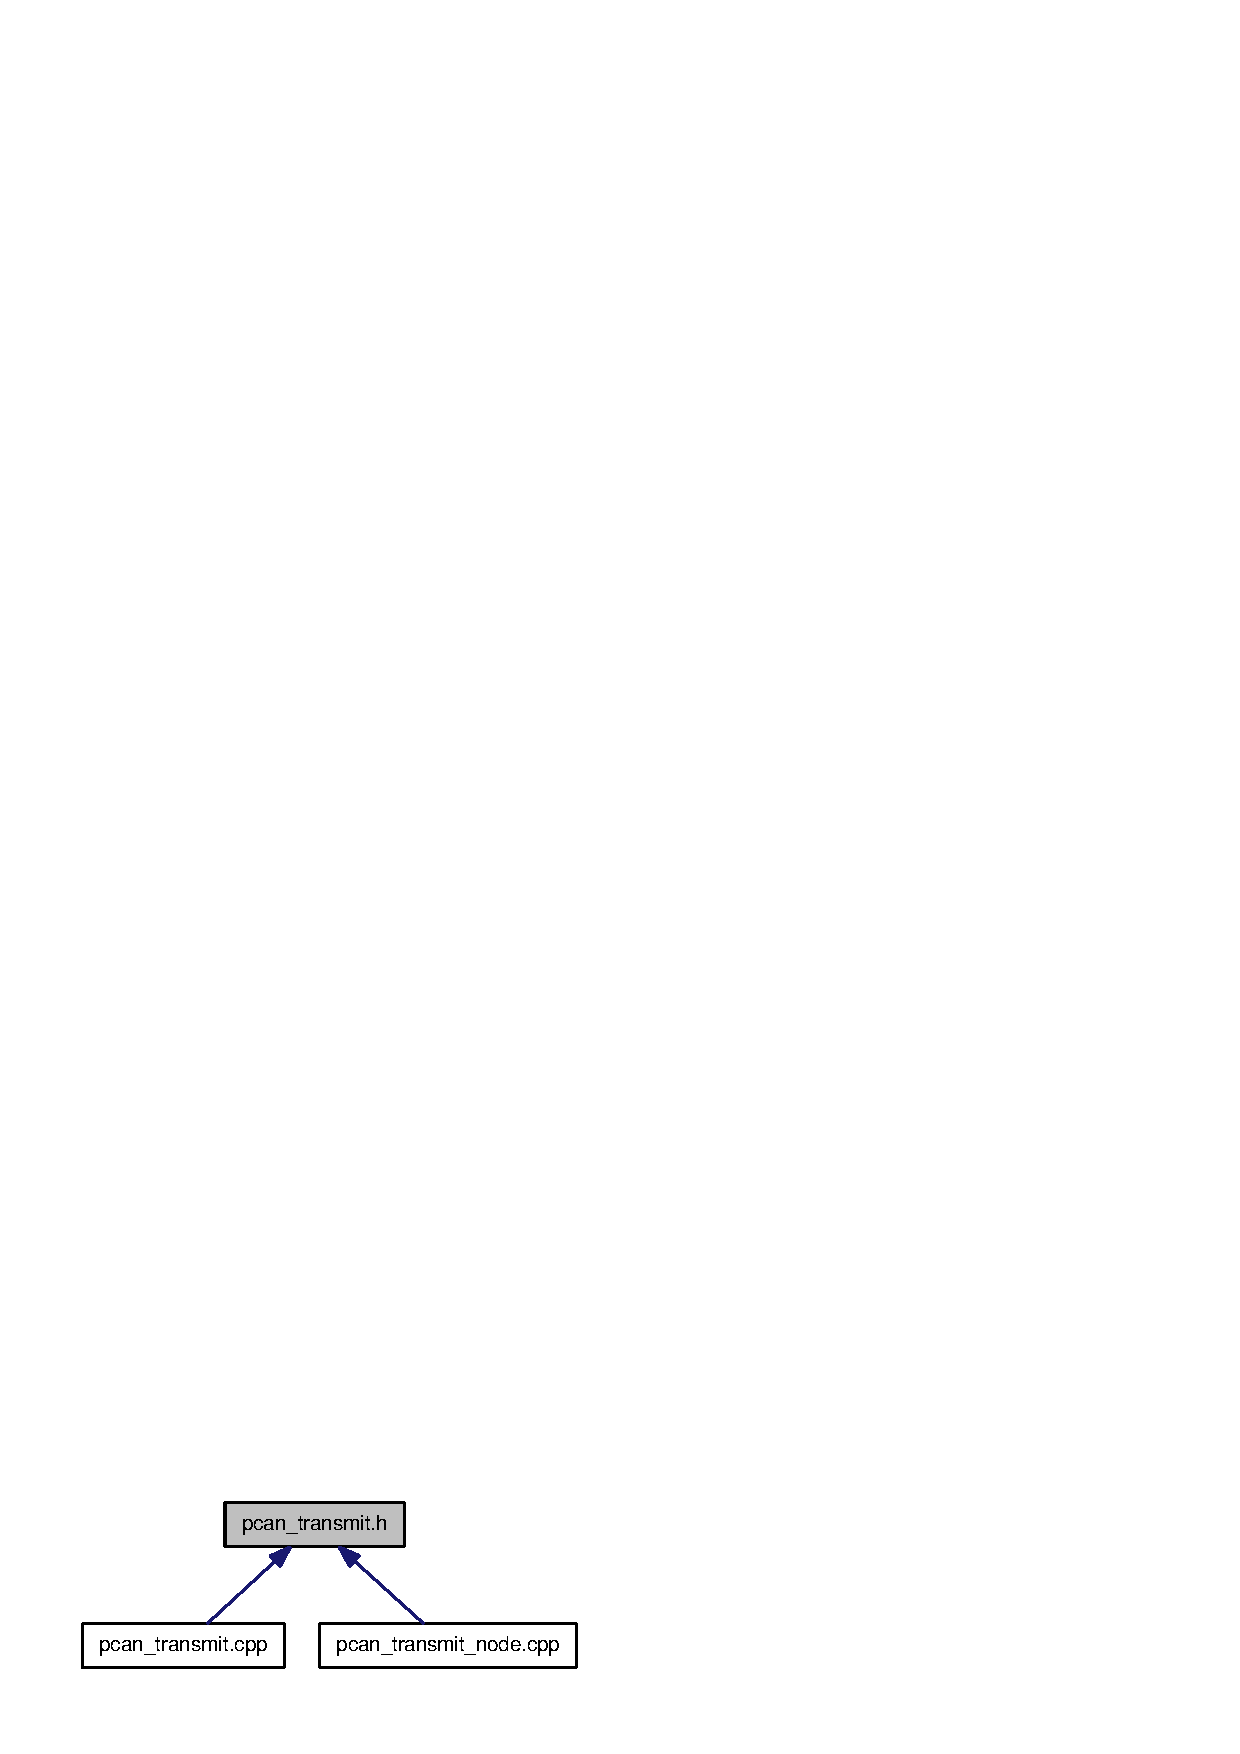
\includegraphics[width=280pt]{pcan__transmit_8h__dep__incl}
\end{center}
\end{figure}
\subsection*{\-Classes}
\begin{DoxyCompactItemize}
\item 
class {\bf pcan\-\_\-transmit}
\end{DoxyCompactItemize}
\subsection*{\-Defines}
\begin{DoxyCompactItemize}
\item 
\#define {\bf \-C\-U\-R\-R\-E\-N\-T\-\_\-\-R\-E\-L\-E\-A\-S\-E}~\char`\"{}\-Release\-\_\-20090203\-\_\-n\char`\"{}
\item 
\#define {\bf \-D\-E\-F\-A\-U\-L\-T\-\_\-\-N\-O\-D\-E}~\char`\"{}/dev/pcan32\char`\"{}
\end{DoxyCompactItemize}


\subsection{\-Define \-Documentation}
\index{pcan\-\_\-transmit.\-h@{pcan\-\_\-transmit.\-h}!\-C\-U\-R\-R\-E\-N\-T\-\_\-\-R\-E\-L\-E\-A\-S\-E@{\-C\-U\-R\-R\-E\-N\-T\-\_\-\-R\-E\-L\-E\-A\-S\-E}}
\index{\-C\-U\-R\-R\-E\-N\-T\-\_\-\-R\-E\-L\-E\-A\-S\-E@{\-C\-U\-R\-R\-E\-N\-T\-\_\-\-R\-E\-L\-E\-A\-S\-E}!pcan_transmit.h@{pcan\-\_\-transmit.\-h}}
\subsubsection[{\-C\-U\-R\-R\-E\-N\-T\-\_\-\-R\-E\-L\-E\-A\-S\-E}]{\setlength{\rightskip}{0pt plus 5cm}\#define {\bf \-C\-U\-R\-R\-E\-N\-T\-\_\-\-R\-E\-L\-E\-A\-S\-E}~\char`\"{}\-Release\-\_\-20090203\-\_\-n\char`\"{}}\label{pcan__transmit_8h_a83a4c9c8303948a33b0bc5050142643a}


\-Definition at line 21 of file pcan\-\_\-transmit.\-h.

\index{pcan\-\_\-transmit.\-h@{pcan\-\_\-transmit.\-h}!\-D\-E\-F\-A\-U\-L\-T\-\_\-\-N\-O\-D\-E@{\-D\-E\-F\-A\-U\-L\-T\-\_\-\-N\-O\-D\-E}}
\index{\-D\-E\-F\-A\-U\-L\-T\-\_\-\-N\-O\-D\-E@{\-D\-E\-F\-A\-U\-L\-T\-\_\-\-N\-O\-D\-E}!pcan_transmit.h@{pcan\-\_\-transmit.\-h}}
\subsubsection[{\-D\-E\-F\-A\-U\-L\-T\-\_\-\-N\-O\-D\-E}]{\setlength{\rightskip}{0pt plus 5cm}\#define {\bf \-D\-E\-F\-A\-U\-L\-T\-\_\-\-N\-O\-D\-E}~\char`\"{}/dev/pcan32\char`\"{}}\label{pcan__transmit_8h_a7ce36d8e87af0db87c0d228a64201e35}


\-Definition at line 20 of file pcan\-\_\-transmit.\-h.


\section{pcan\-\_\-transmit\-\_\-node.\-cpp \-File \-Reference}
\label{pcan__transmit__node_8cpp}\index{pcan\-\_\-transmit\-\_\-node.\-cpp@{pcan\-\_\-transmit\-\_\-node.\-cpp}}
{\ttfamily \#include $<$stdio.\-h$>$}\*
{\ttfamily \#include $<$stdlib.\-h$>$}\*
{\ttfamily \#include $<$errno.\-h$>$}\*
{\ttfamily \#include $<$unistd.\-h$>$}\*
{\ttfamily \#include $<$signal.\-h$>$}\*
{\ttfamily \#include $<$string.\-h$>$}\*
{\ttfamily \#include $<$fcntl.\-h$>$}\*
{\ttfamily \#include $<$libpcan.\-h$>$}\*
{\ttfamily \#include $<$ctype.\-h$>$}\*
{\ttfamily \#include \char`\"{}common.\-h\char`\"{}}\*
{\ttfamily \#include \char`\"{}pcan\-\_\-transmit.\-h\char`\"{}}\*
{\ttfamily \#include \char`\"{}ros/ros.\-h\char`\"{}}\*
{\ttfamily \#include \char`\"{}std\-\_\-msgs/\-String.\-h\char`\"{}}\*
{\ttfamily \#include $<$sstream$>$}\*
\-Include dependency graph for pcan\-\_\-transmit\-\_\-node.\-cpp\-:\nopagebreak
\begin{figure}[H]
\begin{center}
\leavevmode
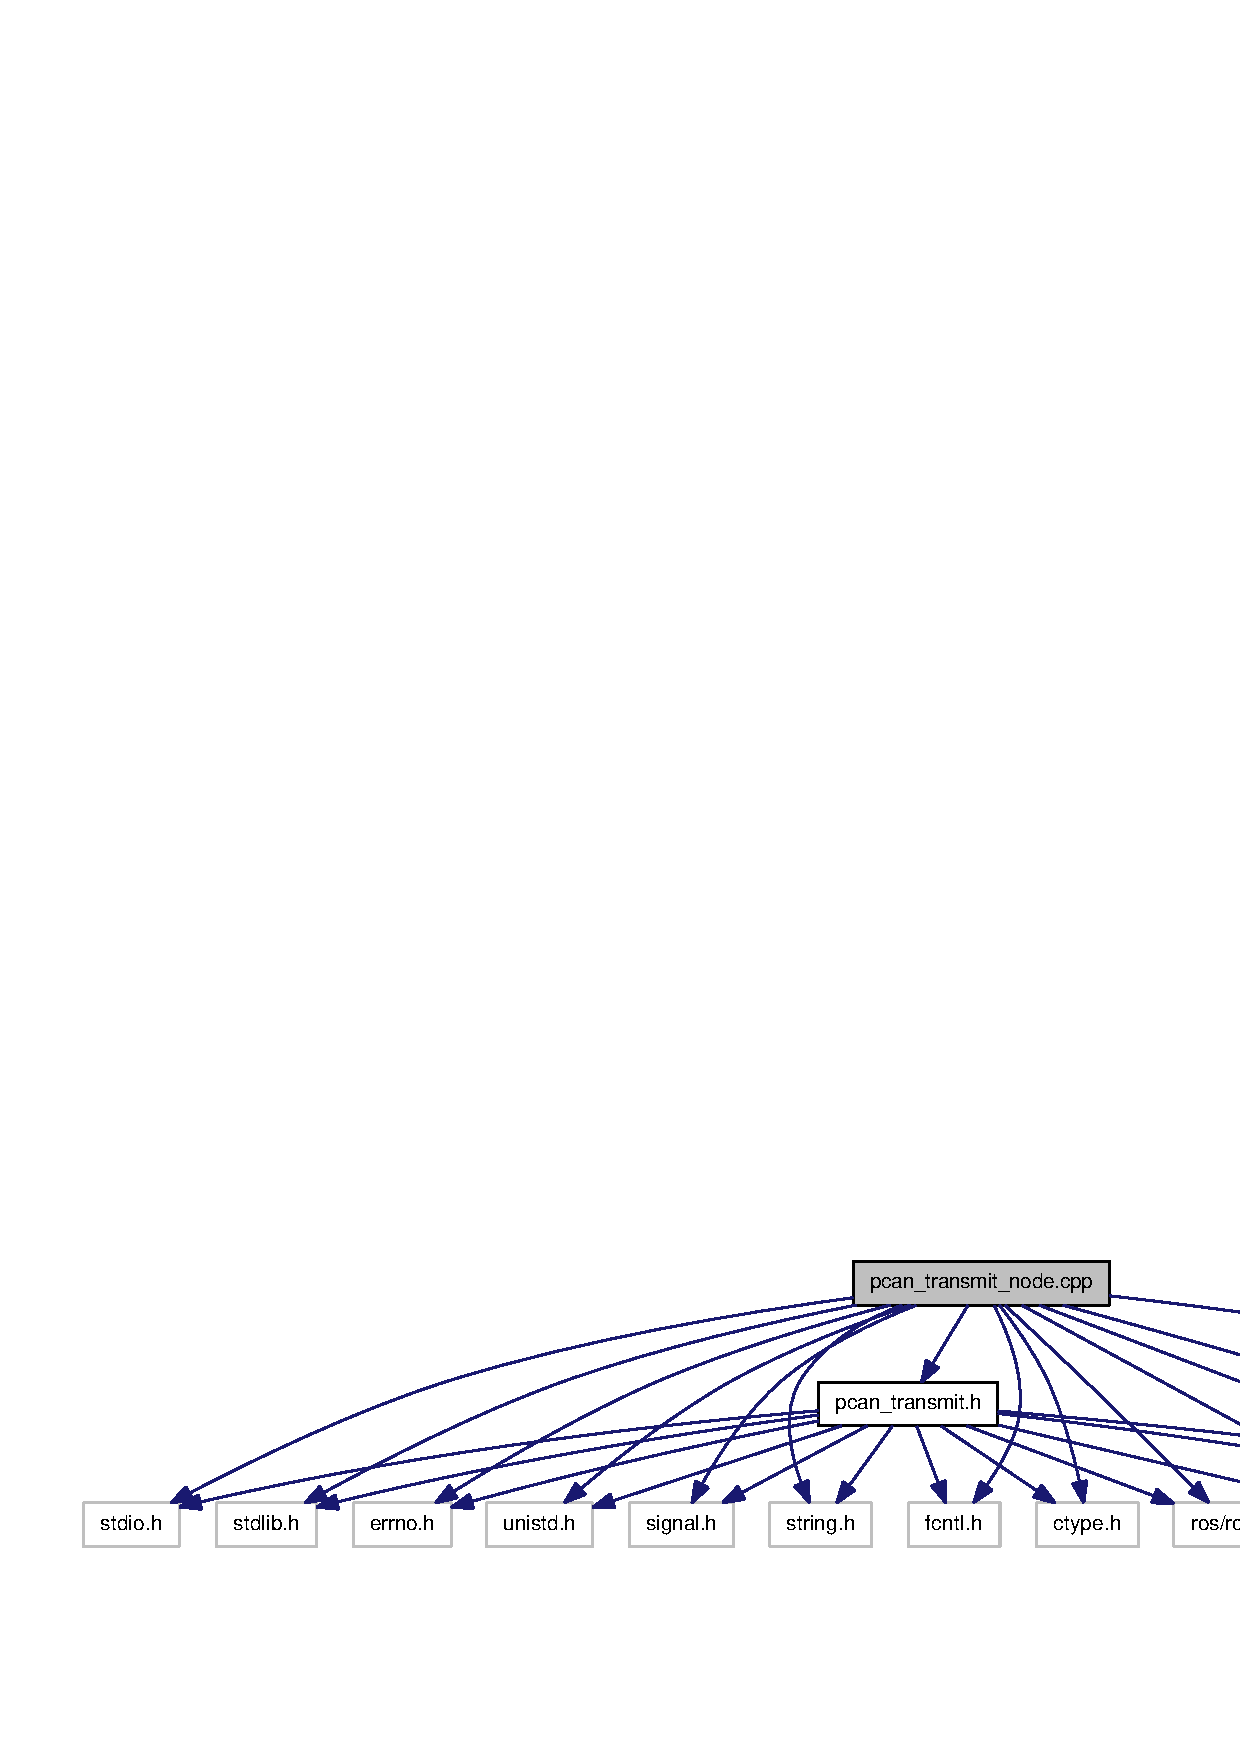
\includegraphics[width=350pt]{pcan__transmit__node_8cpp__incl}
\end{center}
\end{figure}
\subsection*{\-Defines}
\begin{DoxyCompactItemize}
\item 
\#define {\bf \-C\-U\-R\-R\-E\-N\-T\-\_\-\-R\-E\-L\-E\-A\-S\-E}~\char`\"{}\-Release\-\_\-20090203\-\_\-n\char`\"{}
\item 
\#define {\bf \-D\-E\-F\-A\-U\-L\-T\-\_\-\-N\-O\-D\-E}~\char`\"{}/dev/pcan32\char`\"{}
\end{DoxyCompactItemize}
\subsection*{\-Functions}
\begin{DoxyCompactItemize}
\item 
int {\bf main} (int argc, char $\ast$$\ast$argv)
\end{DoxyCompactItemize}
\subsection*{\-Variables}
\begin{DoxyCompactItemize}
\item 
const char $\ast$ {\bf current\-\_\-release}
\item 
\-H\-A\-N\-D\-L\-E {\bf h}
\end{DoxyCompactItemize}


\subsection{\-Define \-Documentation}
\index{pcan\-\_\-transmit\-\_\-node.\-cpp@{pcan\-\_\-transmit\-\_\-node.\-cpp}!\-C\-U\-R\-R\-E\-N\-T\-\_\-\-R\-E\-L\-E\-A\-S\-E@{\-C\-U\-R\-R\-E\-N\-T\-\_\-\-R\-E\-L\-E\-A\-S\-E}}
\index{\-C\-U\-R\-R\-E\-N\-T\-\_\-\-R\-E\-L\-E\-A\-S\-E@{\-C\-U\-R\-R\-E\-N\-T\-\_\-\-R\-E\-L\-E\-A\-S\-E}!pcan_transmit_node.cpp@{pcan\-\_\-transmit\-\_\-node.\-cpp}}
\subsubsection[{\-C\-U\-R\-R\-E\-N\-T\-\_\-\-R\-E\-L\-E\-A\-S\-E}]{\setlength{\rightskip}{0pt plus 5cm}\#define {\bf \-C\-U\-R\-R\-E\-N\-T\-\_\-\-R\-E\-L\-E\-A\-S\-E}~\char`\"{}\-Release\-\_\-20090203\-\_\-n\char`\"{}}\label{pcan__transmit__node_8cpp_a83a4c9c8303948a33b0bc5050142643a}


\-Definition at line 22 of file pcan\-\_\-transmit\-\_\-node.\-cpp.

\index{pcan\-\_\-transmit\-\_\-node.\-cpp@{pcan\-\_\-transmit\-\_\-node.\-cpp}!\-D\-E\-F\-A\-U\-L\-T\-\_\-\-N\-O\-D\-E@{\-D\-E\-F\-A\-U\-L\-T\-\_\-\-N\-O\-D\-E}}
\index{\-D\-E\-F\-A\-U\-L\-T\-\_\-\-N\-O\-D\-E@{\-D\-E\-F\-A\-U\-L\-T\-\_\-\-N\-O\-D\-E}!pcan_transmit_node.cpp@{pcan\-\_\-transmit\-\_\-node.\-cpp}}
\subsubsection[{\-D\-E\-F\-A\-U\-L\-T\-\_\-\-N\-O\-D\-E}]{\setlength{\rightskip}{0pt plus 5cm}\#define {\bf \-D\-E\-F\-A\-U\-L\-T\-\_\-\-N\-O\-D\-E}~\char`\"{}/dev/pcan32\char`\"{}}\label{pcan__transmit__node_8cpp_a7ce36d8e87af0db87c0d228a64201e35}


\-Definition at line 21 of file pcan\-\_\-transmit\-\_\-node.\-cpp.



\subsection{\-Function \-Documentation}
\index{pcan\-\_\-transmit\-\_\-node.\-cpp@{pcan\-\_\-transmit\-\_\-node.\-cpp}!main@{main}}
\index{main@{main}!pcan_transmit_node.cpp@{pcan\-\_\-transmit\-\_\-node.\-cpp}}
\subsubsection[{main}]{\setlength{\rightskip}{0pt plus 5cm}int {\bf main} (
\begin{DoxyParamCaption}
\item[{int}]{argc, }
\item[{char $\ast$$\ast$}]{argv}
\end{DoxyParamCaption}
)}\label{pcan__transmit__node_8cpp_a3c04138a5bfe5d72780bb7e82a18e627}
\-The \doxyref{main()}{p.}{pcan__receive__node_8cpp_a3c04138a5bfe5d72780bb7e82a18e627} function only starts a \-R\-O\-S node, creates and initiates a \doxyref{pcan\-\_\-transmit}{p.}{classpcan__transmit} object instance, and starts to spin \-R\-O\-S.

\-Definition at line 29 of file pcan\-\_\-transmit\-\_\-node.\-cpp.



\subsection{\-Variable \-Documentation}
\index{pcan\-\_\-transmit\-\_\-node.\-cpp@{pcan\-\_\-transmit\-\_\-node.\-cpp}!current\-\_\-release@{current\-\_\-release}}
\index{current\-\_\-release@{current\-\_\-release}!pcan_transmit_node.cpp@{pcan\-\_\-transmit\-\_\-node.\-cpp}}
\subsubsection[{current\-\_\-release}]{\setlength{\rightskip}{0pt plus 5cm}const char$\ast$ {\bf current\-\_\-release}}\label{pcan__transmit__node_8cpp_ab70111b16fc3d1e36d0a598452c6f43c}


\-Definition at line 27 of file pcan\-\_\-transmit\-\_\-node.\-cpp.

\index{pcan\-\_\-transmit\-\_\-node.\-cpp@{pcan\-\_\-transmit\-\_\-node.\-cpp}!h@{h}}
\index{h@{h}!pcan_transmit_node.cpp@{pcan\-\_\-transmit\-\_\-node.\-cpp}}
\subsubsection[{h}]{\setlength{\rightskip}{0pt plus 5cm}\-H\-A\-N\-D\-L\-E {\bf h}}\label{pcan__transmit__node_8cpp_a0182b2e472b8af2291079784ca8926c9}


\-Definition at line 26 of file pcan\-\_\-transmit\-\_\-node.\-cpp.


\printindex
\end{document}
